\chapter{Interdisciplinary tree disease epidemics}
\label{chapter2:litreview} 

Understanding modern-day tree disease epidemics requires a holistic, interdisciplinary
approach, made possible only by the convergence of numerous scientific fields. 
Consequently, this Chapter reviews several key modelling themes.
Models of tree disease aim to help design effective control policies and inform policymakers.
Well-informed policymakers can then help to maintain tree health in rural, urban and commercial environments. 
Although myriad environmental, biological and anthropomorphic factors complicate the scientific understanding 
and thus effective disease control. 

Here, the review begins by narrating some early historical developments in human and botanical epidemiology before presenting
a variety of present-day modelling frameworks. After introducing the mainstream paradigm of plant-based epidemic models,
an inspection of dispersal, thresholds, and epidemic control follow naturally. Then, several tree distribution datasets in Great Britain are presented and compared. Finally, the Chapter ends with a case study of ash dieback, reflecting the multi-faceted 
difficulties posed by a recent emergent epidemic.

\newpage

\section{Historical perspectives}

Historically, the fields of plant pathology and mathematical epidemiology existed in different spheres.
Plant pathology researchers furthered biological understanding of pathogen growth (e.g. \cite{doi:10.1146/annurev.py.01.090163.000245}), not predictive mathematical theories.
Although, pioneering discoveries in mathematical epidemiology permitted a more quantitative treatment of botanical diseases. 
In particular, the seminal $SIR$ model of \cite{kermack-model} 
provided a foundation to examine plant-based epidemics mathematically.

\subsection{Standard $SIR$}

The \cite{kermack-model} (K \& M) model involves three compartmentalised fields, 
susceptible $S(t)$, infected $I(t)$ and removed $R(t)$.
Each field models the evolution of a closed population of size $N$, where $N = S(t) + I(t) + R(t)$. 
A coupled system of ODEs then follow:
\begin{align}
\label{eq:SIR-model1}
    &\frac{dS}{dt} = -\beta SI \\
    &\frac{dI}{dt} = \beta SI - \mu I \\
    \label{eq:SIR-model3}
    &\frac{dR}{dt} = \mu I
\end{align}
where the term $\beta S I$ dictates the flow of susceptible hosts into the infected compartment according 
to the rate $\beta$. Likewise, $\mu I$ controls the transition of infected hosts into the removed compartment
through a removal rate $\mu$. Figure \ref{fig:SIR-vs-plank}(a) illustrates the coupled $SIR$ system for 
fixed $\mu$ and four values of $\beta$.

The coupled differential system of Equations (\ref{eq:SIR-model1}-\ref{eq:SIR-model3}) rely on several assumptions, including:
1) a closed population with no births or deaths 2) no exposed/incubation period 3) lifetime immunity following recovery
4) mass action population mixing, where contact mixing rates between individuals in $S$ and $I$ are proportional 
to the number of individuals in either field.

Today, countless articles have relaxed these assumptions to extend the standard $SIR$ framework\footnote{
Indeed, following the COVID-19 pandemic, $SIR$-type models remain an active field of research 
and dominate present-day epidemic literature \cite{atkeson2020using}.}.
Nevertheless, a keystone result emerged from Equations (\ref{eq:SIR-model1}-\ref{eq:SIR-model3}), namely 
the existence of a critical epidemic threshold, captured through either:
\begin{align}
    \label{eq:R0-SIR}
    & R_0 = \frac{\beta}{\mu}\\
    \label{eq:R0-effective}
    & R_e = \frac{S(t)}{N} \frac{\beta}{\mu}
\end{align}
where $R_0$ and $R_c$ are referred to as the basic and effective reproduction numbers, respectively.
Following the introduction of one infected host at $t=0$, $N\sim S(0)$ and 
we have $R_e=\big((N-1)/N\big) \beta / \mu$. Therefore, in the limit of a large population at $t=0$, 
$\big((N-1)/N\big)$ approximates unity and $R_e = R_0$, otherwise $R_e=\big(S(t)/N\big) R_0$.

Both quantities $R_0$ and $R_e$ describe an epidemic threshold, though $R_e$ captures a threshold in the face
of a declining susceptible population by including the ratio $S(t)/N$.
Equation \ref{eq:R0-effective} defines a critical threshold by the simple criterion\footnote{
For a more comprehensive mathematical proof of $SIR$
model thresholds, the reader is directed towards \cite{weiss2013sir}}:
1) when $R_e > 1$, then $I(t)$ rises sharply, culminating in an epidemic before declining in the absence of newly
infected hosts
2) if $R_e \leq 1$, then $I(t)$ quickly declines to zero as $t\rightarrow 0$ and the outbreak subsides.


\subsection{Logistic growth}
\label{sec:logistic-growth}
The seminal work of \cite{van2013plant} firmly established ties between plant pathology and 
mathematical epidemiology.
Fundamentally, Van der Plank equated the growth of plant pathogens (or `inoculum') to logistic growth of the form:
\begin{equation}
    \label{van-plank}
    \frac{dI}{dt} = rI(1 - I)
\end{equation}
where $r$ describes the rate of pathogen growth and $I$ reflects the proportion of infected tissue.
In Equation \ref{van-plank}, the amount of infected tissue $I$ snowballs at first, 
in proportion to the amount of inoculum. Then, as time passes and $I$ grows, $(1-I)$ approximates zero, 
and the system plateaus as all susceptible tissue becomes infected.
The essential model behaviour is shown in Figure \ref{fig:SIR-vs-plank}(b) over $10$ values growth rates $r$.
From Equation \ref{van-plank}, a simple method to determine the rate $r$ follows:
\begin{equation}
    \label{eq:van-plank-r}
    r =\frac{1}{t_2 - t_1} \log \Big(\frac{I_2}{1 - I_2} - \frac{I_1}{1 - I_1}\Big)
\end{equation}
where $I_1$ and $I_2$ are the proportions of infected tissue at times $t_1$ and $t_2$ respectively\textemdash 
see \cite{van2013plant} Chapter 3. Importantly, both $I_1$ and $I_2$, and by extension the infection rate $r$,
are measurable in laboratory conditions. 
In Equation \ref{van-plank}, newly infected tissue becomes infectious immediately following infection.
Realistically, infectious tissue (and symptom expression) takes time to develop, described by an `incubation period'.
Accordingly, Van der Plank adapted Equation \ref{van-plank} to a delay differential equation (DDE):
\begin{equation}
\label{van-plank-incubation}
    \frac{dI_t}{dt} = RI_{t-p}(1 - I_{t})
\end{equation}
where $I_t$ and $I_{t-p}$ describe the infectious tissue at times $t$ and $t-p$ and $p$ is the incubation period. 
Hence, infectious tissue grows in response to the factor $R I_{t-p}$, and saturates
according to the logistic term $(1 - I_t)$. The parameter $R$ now describes pathogen
growth at step $t-p$, as opposed to $r$ that describes the spread of disease at step $t$, leading to the ratio:
\begin{equation}
    \frac{R}{r} = \frac{x_t}{x_{t-p}}
\end{equation}
\begin{figure}
     \centering
     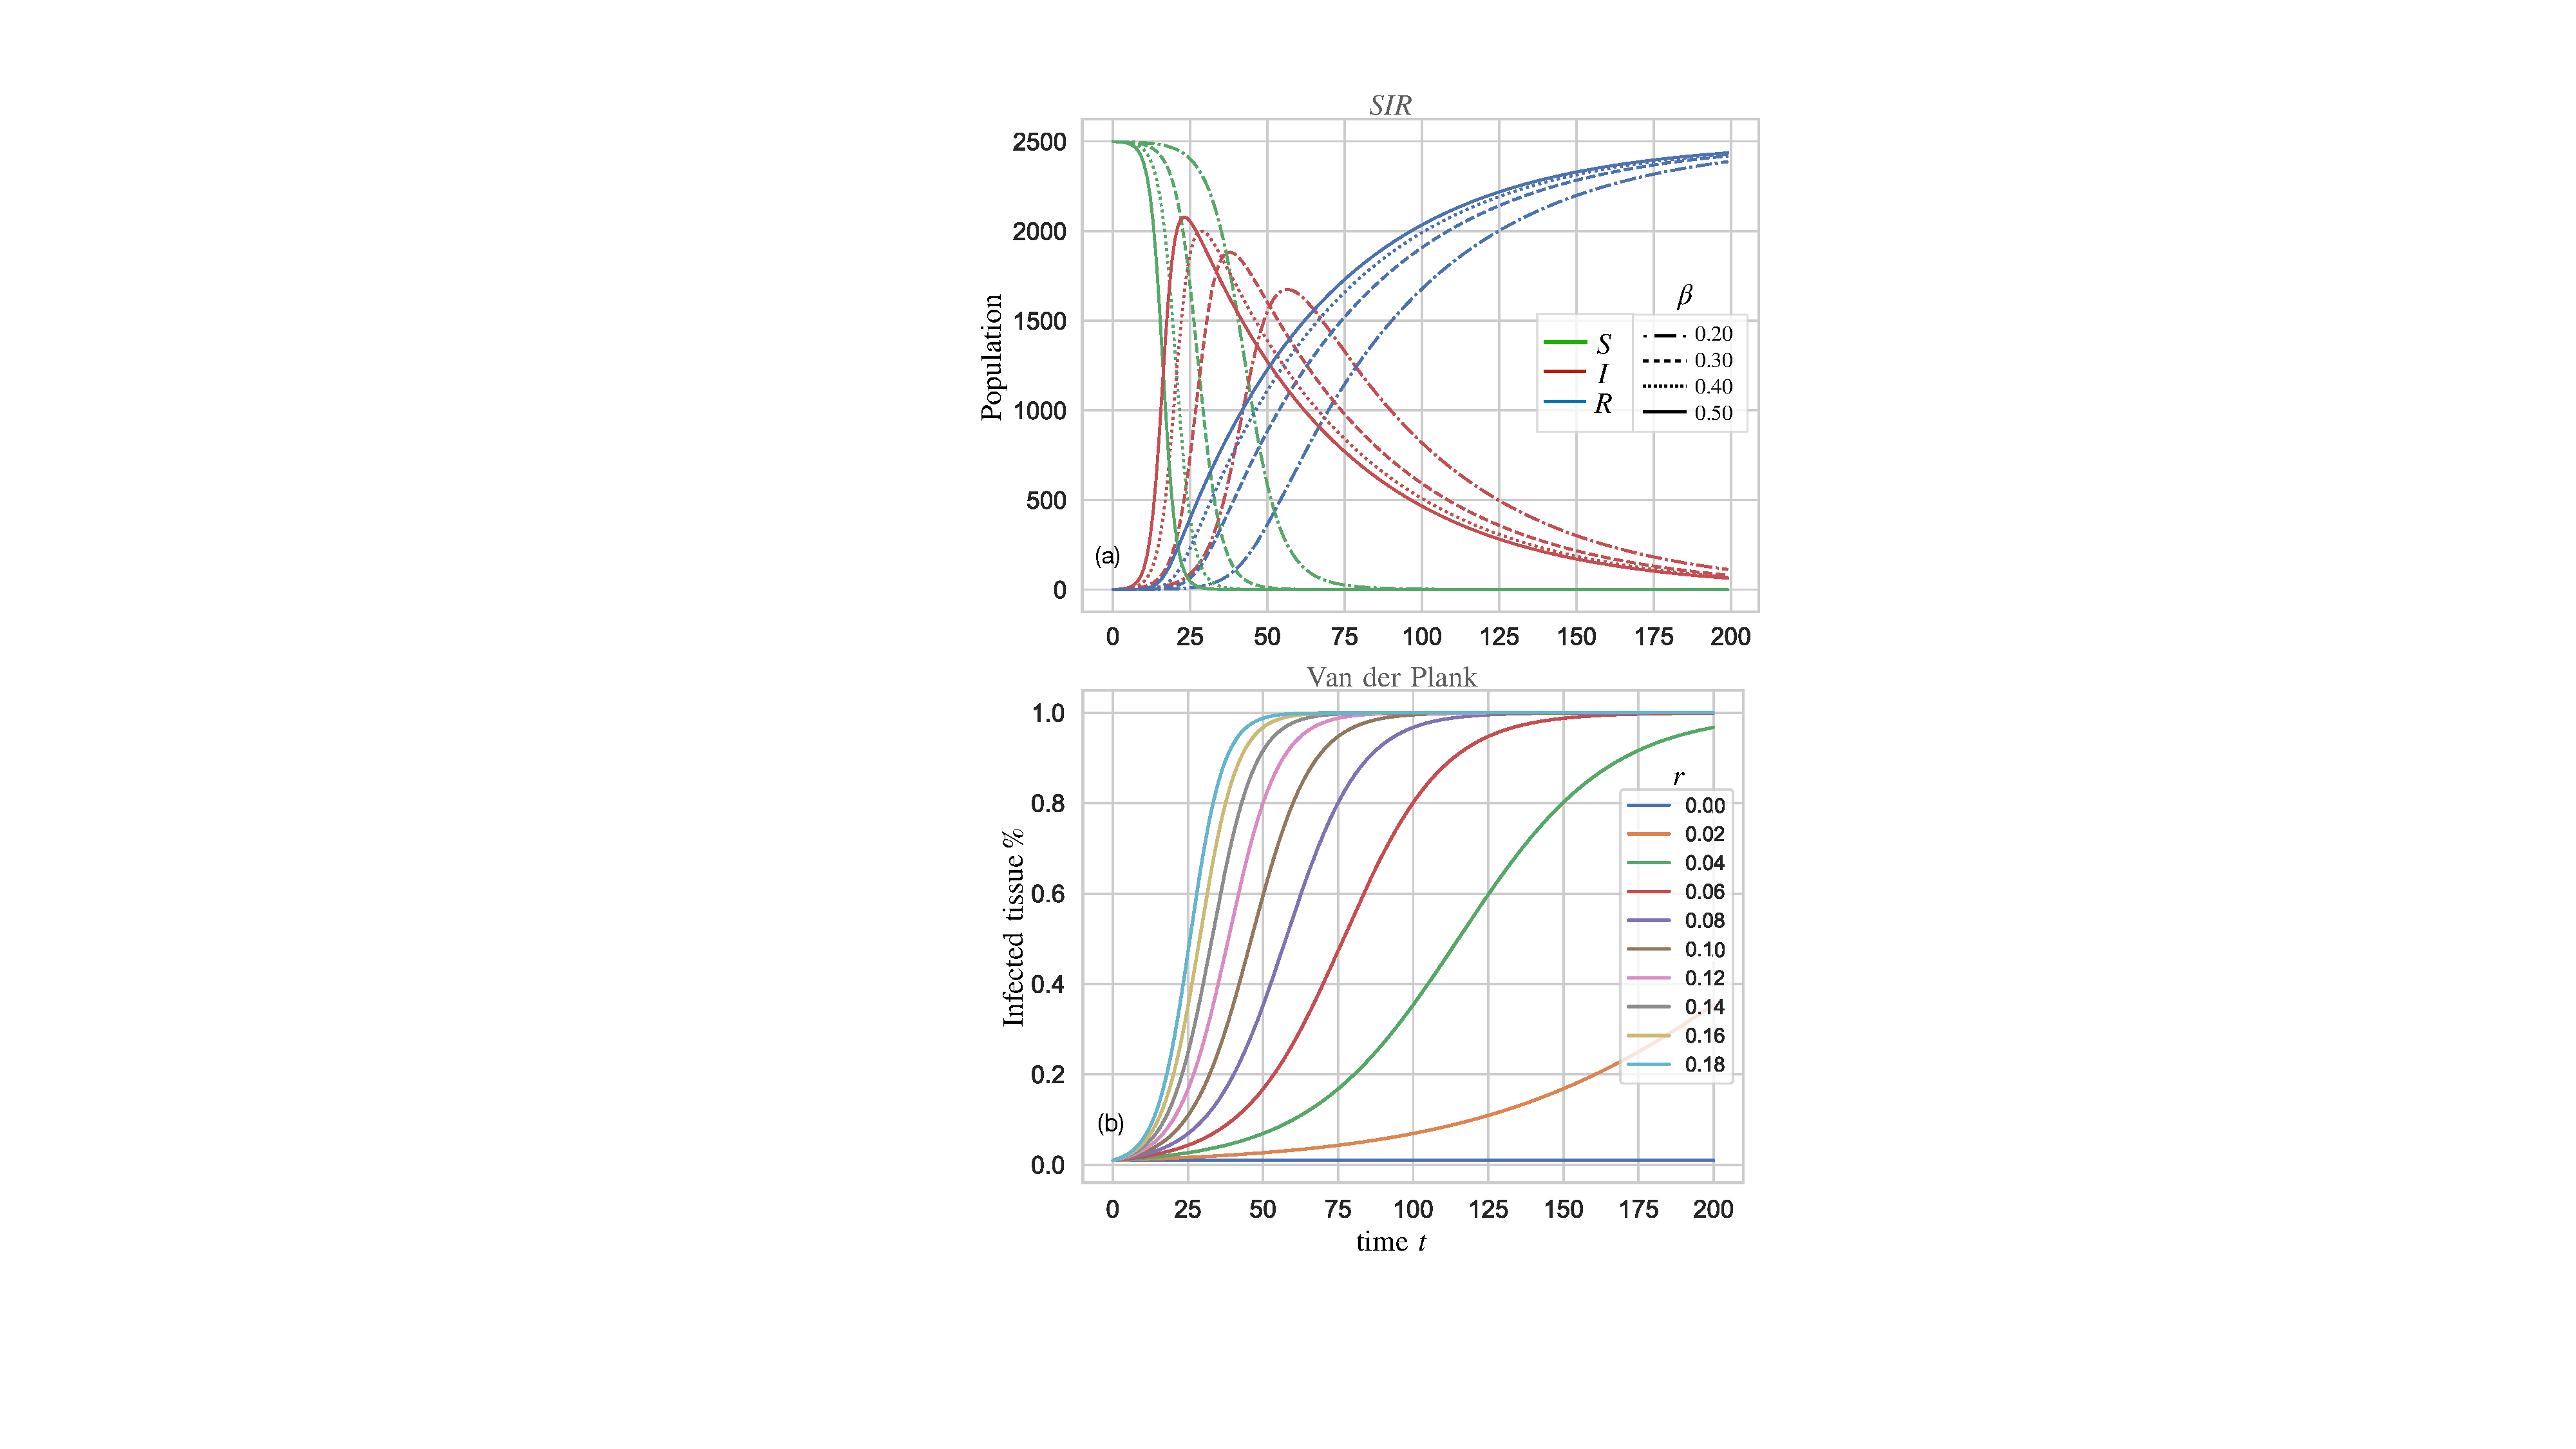
\includegraphics[scale=0.55]{chapter2/figures/SIR-vs-Plank.pdf}
     \caption{(a) The $SIR$ model as presented by \cite{kermack-model} is shown for fixed removal rate $\mu = 0.20$ and variations of $\beta$. 
                  The coupled system of ODEs can be solved numerically with Euler's method. Here, simulations begin with 
                  $2500$ susceptible and one infected individuals, and evolve for $t=200$ steps.
                  (b) The logistic growth model \cite{van2013plant} used to describe the growth of infected plant material.
                  Simulations are numerically computed with a forward-time finite difference method for $10$ different growth rates $r$.
       } 
     \label{fig:SIR-vs-plank}
 \end{figure}
where $r$ represents an `apparent' infection rate (measurable in laboratories from Equation \ref{eq:van-plank-r}),
and $R$ denotes the `basic' infection rate. As Plank explained, one usually seeks
to determine $R$ from the constant $r$. Assuming that $r$ indeed stays constant over the epidemic:
the basic infection rate $R$ must decrease as $x_t/x_{t-p}$ gets progressively smaller as $x_{t-p}\rightarrow x_t $.
At this point, the basic infection rate $R$ begins to resemble the effective reproduction ratio $R_e$
from Equation \ref{eq:R0-effective}. 

Equation \ref{van-plank-incubation} describes a system where
infections incubate for a period $p$ before inducing the growth of more infectious plant tissue.
However, it does not describe the infectious period (where infected tissue remains before becoming epidemiologically inert),
which lead Plank to extend Equation \ref{van-plank-incubation} to:
\begin{equation}
\label{van-plank-infectious-p}
    \frac{dI_t}{dt} = R_c(I_{t-p} - I_{t-i-p})(1 - I_{t})
\end{equation}
where $R_c$ is the basic infection rate `corrected' for removals and $i$ is the infectious period.
In this DDE, a unit of latently infectious tissue starts becoming infectious after $p$ steps, and stops becoming infectious $i$ steps.
More formally, as $I_{t-i-p} \rightarrow I_{t-p}$, the rate of infectious tissue growth approaches zero, $dI_t/dt \rightarrow 0$.

\subsection{Contrasting approaches}
\label{sec:SIR-vs-plank}

The $SIR$ model does not include an incubation period, and therefore differs from the delayed differential formulation 
of Equation \ref{van-plank-infectious-p}. Nonetheless, the compartmentalised approach is easy to extend, leading to an 
$SEIR$ system:
\begin{align}
\label{eq:SEIR-model1}
    &\frac{dS}{dt} = -\beta SI \\
\label{eq:SEIR-model2}
    &\frac{dE}{dt} = \beta SI - \gamma E\\
    &\frac{dI}{dt} = \gamma E - \mu I \\
    \label{eq:SEIR-model3}
    &\frac{dR}{dt} = \mu I
\end{align}
where Equation \ref{eq:SEIR-model2} describes the population of latently (or exposed) infected hosts.
Susceptible hosts transition into the exposed compartment at the same rate as before, namely $\beta SI$, but now have an
exponentially distributed latency period of $\gamma^{-1}$ before transitioning into $I$.

Both Equations \ref{eq:SEIR-model1}-\ref{eq:SEIR-model3} and Equation \ref{van-plank-infectious-p} outline similar systems,
though infected tissue in Equation \ref{van-plank-infectious-p} remains infectious for precisely $i$ units.
This contrasts with the exponentially distributed exposed lifetime implicit within Equation \ref{eq:SEIR-model2}.
Nevertheless, \cite{segarra2001epidemic} illustrated how Plank's DDE and the $SEIR$ system are both special cases of
the $SIR$ model proposed by \cite{kermack-model}, when the $SIR$ model incorporates a sporulation function, $\phi(\tau)$. 
The sporulation function appropriately models spore production in plant pathogens. 
In particular, if $\phi(\tau) = 0$ for small $t$, $\phi(\tau)$ can model incubation periods. 
Similarly, if $\phi(\tau) = 0$  for large $t$, we recover an infectious period. 
More recently, \cite{time-varying-infectivity} simplified the analysis of \cite{segarra2001epidemic}, showing that 
both Plank's DDE and the $SEIR$ model can be recovered with an $SE_nI_mR$ model.
In an $SE_nI_mR$ framework, both $n$ and $m$ represent an arbitrary number of distinct exposed and infectious compartments:
\[
    S\rightarrow E_1 \rightarrow E_2 \rightarrow ... \rightarrow E_n \rightarrow I_1 \rightarrow I_2 \rightarrow ... I_m
\]
Trivially, the $SEIR$ model is recovered when $n=1$ and $m=1$. However, when $n,m \rightarrow \infty$,
\cite{time-varying-infectivity} demonstrated that we recover an expression equivalent to the DDE in Equation \ref{van-plank-infectious-p}.
Despite the sameness of both DDE and $SEIR$ formulations, the overarching theme of modern epidemiology is overwhelmingly compartmentalised,
owing to the increased flexibility and easier analysis of compartmental models.


\subsection{Progressive botanical epidemiology}
\label{sec:prog-epi}
After \cite{van2013plant} moved the field of botanical diseases into a more quantitative discipline,
theoretical investigations (alongside the adoption of computer simulations) characterised the next few decades.
Plank's DDE was applied to numerous pathosystems, halo blight in beans \cite{doi:10.1111/j.1744-7348.1979.tb06527.x} 
and grape powdery mildew \cite{sall1980epidemiology} to name a few. In particuar, \cite{sall1980epidemiology} adapted Plank's
logistic approach to include a time-varying infection rate $r(t)$. Moreover, diverse mathematical techniques, 
including multiple  regression analysis, were incorporated into mainstream plant epidemiology \cite{butt1974multiple}. 
Subsequently, \cite{zadoks1979epidemiology} consolidated various early mathematical models of plant disease 
alongside \cite{jeger1984use}.

Developments in computing compounded advances in plant epidemiology through this period. 
Improved accessibility and computer architectures permitted faster calculations and more intensive models. 
The first epidemic simulator (EPIDEM) written in FORTRAN IV came by \cite{waggoner1969epidem}. 
EPIDEM modelled the fungi `Alternaria solani' spreading through infected potato and tomato leaf tissue under different environmental conditions. 
    
An interesting early simulator (EPIMUL76) developed by \cite{zadoks1977role} adapted Van der Plank's logistic growth model into a spatio-temporal framework of two spatial dimensions. 
EPIMUL76 simulated the spread of disease on a two-dimensional domain, subdivided into $20\times 20$ host units referred to as `compartments', that took place inside a computer with $128\mathrm{K}$ of memory.
Arguably, subdividing the domain into separate compartments could be considered as an early agent-based model. 

In their analysis, \cite{zadoks1977role} alluded to the problem of scale in plant disease, as spatial scales
were conceptualised as `microscales' ($\leq 1\mathrm{m}$), `mesoscales' ($10^2\mathrm{m}$) and `macroscales' ($10^6\mathrm{m}$).
In this picture, microscales ranged from plant leaves to individual plants, mesoscales reflected crop fields, and macroscales
described large regional expanses over an entire country. Moreover, the probability of dispersal between infected hosts assumed a
Gaussian distribution\textemdash in contrast to \cite{doi:10.1146/annurev.py.06.090168.001201}.

In general, the ability to simulate more intricate models grew in proportion to the amount of computer memory available.
For a review of early plant disease simulators, see \cite{doi:10.1146/annurev.py.23.090185.002031}.

\subsection{Percolation: from forest fires to epidemics}
\label{section:lit-rev-perc}

Research on percolation occurred alongside the developing field of plant disease modelling.
The development of percolation theory marked an early approach to modelling epidemic systems that are
both spatially-explicit and stochastic.
The original formulation of percolation theory was first used to describe properties of a fluid and the 
bonds that form between molecules \cite{perco_origin} (a more formal description of 
percolation is undertaken later in section \ref{sec:perc-form}). The problem was posed on a 
graph\textemdash illustrated in terms of vertices and edges. However re-interpretations were subsequently 
put forward by physicists studying material sciences, naturally on a lattice. \cite{Essam_1980}. 
An attractive feature outlined by this new approach was a phase-transition that could be treated with scaling theory\textemdash
used in the study of critical-phenomena. 
Accordingly, early work rigorously ensued to map out the behaviour of percolation around criticality in 
terms of critical exponents \cite{STAUFFER19791}. 

Different flavours of percolation models, such as site or bond percolation, were described
to model different processes. Nevertheless, percolation proved a convenient theory and various phenomena including gelation, 
magnetism and telecommunications were described \cite{trove.nla.gov.au/work/26493727}. 
With only a short conceptual jump from time-dependent percolation used to study the growth of crystals \cite{Family_1985},
forest fire models were subsequently related to percolation \cite{MacKay_1984}.

Beginning with the $SIR$ framework, mathematical epidemiology was already well-established
around the time percolation theory was conceived \cite{baily1975mathematical}. 
A fire spreading through a population of trees is not too different to a disease spreading through 
a population. Hence, a general percolation-based epidemic-formalisation framework was put forward by
\cite{pub.1059067807}. The researchers proposed that epidemics might be in the same universality class
as percolation.

A fractal-like pattern of epidemics was observed by \cite{GRASSBERGER1986273}, shown in Figure \ref{fig:1d_perc_basis}. 
In Figure \ref{fig:1d_perc_basis}, lighter grey sites represent removed individuals, 
black sites indicate actively infected sites, and white sites indicate unaffected sites. 
All lattice sites in the bottom row were initially infected, and the infection can be seen to propagate
from the bottom up. The lattice was initialised at the critical-density $p\sim p_c$ culminating in a fractal-like pattern.
\cite{GRASSBERGER1986273} did not attribute the hosts of this model to be trees, but instead a general host-population with low mobility. 
The authors noted that local interactions between hosts and infected were vast simplifications and proposed 
generalising the system with long-range interactions following a power law. 
Although, it must be remarked that including long-range interactions would cease to describe a percolation based system.

\begin{figure}
    \centering
    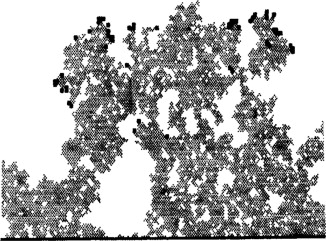
\includegraphics{chapter2/figures/perc1.jpg}
    \caption{A space-time representation of an epidemic spreading at the critical threshold. 
    The spatial (horizontal) and time (vertical) axis show self-similar propagation of diseased 
    individuals in grey, produced by \cite{GRASSBERGER1986273}}
    \label{fig:1d_perc_basis}
\end{figure}

Percolation models of epidemics were examined in several contexts,
including renormalisation-groups \cite{pub.1060474189} and Monte-Carlo methods \cite{pub.1059069981}. 
Studies generally focused on finding the systems critical exponents and categorising phase
transition graph that characterised an epidemic (super-critical) or extinction (sub-critical) 
regimes \cite{GRASSBERGER1986273}. The properties of both epidemics and forest fire percolation 
models were studied together in \cite{pub.1052857560}, highlighting their similarity.

An early ecological applications of percolation was put forward by \cite{pub.1031591030}, 
who studied the effects of landscape distributions and percolation models 
(reflecting both forest fire and tree disease epidemics). In their study, \cite{pub.1031591030} 
combined $SIR$-like mechanics inside a percolation-based distribution of hosts and subsequently 
found a narrow regime where disease epidemics would spread, thus mirroring the threshold-like 
behaviour witnessed in the $SIR$ model. Although, here, the authors considered the possibility of host recovery.
% \textemdash \cite{GRASSBERGER1983157} <- reference for early considerations towards percolation as a model for tree diseases and percolation
% \textemdash \cite{SANDER2002293}, read and get more info + research links
\newpage

\section{Spatially-explicit epidemic models}
\label{ch2:lit-rev-compartmentalised-models}

Emergent infectious diseases (\acrshort{eid}s) in tree populations are multi-scale,
they can span regional, country or continental spatial scales. Considerable variations in landscape composition,
tree densities, population aggregation, and the climatic factors give rise to diverse spatio-temporal
patterns of disease spread \cite{he2019integrating, suzuki2003spatial}. Incorporating spatial structure
into tree disease models is therefore vital to accurately capture environmental influences, host-pathogen 
interactions and dispersal \cite{liu2007characterizing}. This section outlines several approaches to modelling
the spread of tree disease over small, large and multiple spatial scales.

\subsection{Small-scale: stochastic dispersal}
\label{ch2:dispersal}

Pathogen dispersal through wind, watercourse or human trade underpins a key feature of EDIs. 
Numerous functions have been used to model dispersal, but generally, all describe a continuous 
non-negative (real-valued) function that is normalisable: $\int_{-\infty}^{\infty}  D(x)dx = 1$.
Various review articles provide comprehensive functional examples \cite{bullock2017synthesis, nathan2012dispersal, howe1982ecology}.
However, the general class of dispersal kernels include thin-tailed Gaussian and 
exponential alongside fat-tailed inverse power law variants.

Early plant disease simulators (e.g. EPIDEM and EPIMUL76) included stochastic dispersal\textemdash 
discussed at length in section \ref{sec:prog-epi}. A more recent article by \cite{parnell2010effect} 
modelled stochastic dispersal in Citrus canker to investigate the effects of landscape aggregation 
patterns and disease progression.
\cite{parnell2010effect} studied landscape patterns of two kinds: 
1) varying degrees of randomly distributed densities 
2) varying degrees of host aggregation.
The epidemic model was based on a series of prior Citrus canker works
\cite{parnell2009optimal, gilligan2008epidemiological, cook2008constructing}.
The epidemic model is described by:
\begin{equation}
\label{eq:prob-trans}
    Pr(S_i \rightarrow I_i)_{\Delta t} = 1 - \exp\big[- \beta \sum_j^N\exp^{-\alpha d_{ij}} + \epsilon \big]
\end{equation}
Here, a transition probability describes the $i^{th}$ susceptible tree becoming infected 
during the step $t \rightarrow t + \Delta t$ on account of $N$ infected trees.
Equation \ref{eq:prob-trans} assumes that dispersal exponentially decreases with distance (i.e. $\exp^{-\alpha d_{ij}}$), 
where $\alpha$ denotes the dispersal scale parameter. Infection pressure from the $j^{th}$ infected tree is multiplied by an
infection rate, $\beta$. The last parameter to consider in Equation \ref{eq:prob-trans}
is the primary infection rate $\epsilon$. The primary infection rate reflects the chance of infection from sources outside
the immediate system, i.e. at time $t=0$, distant infected populations external to the
closed host population under consideration.

The outside exponential term of Equation \ref{eq:prob-trans} depicts a cumulative exponential threshold above which 
trees become infected. Interestingly, this threshold is based on the `Skelle construction' \cite{sellke1983asymptotic}. 
More specifically, Skelle assumed that susceptive hosts need an arbitrary (cumulative) degree of infection
exposure before becoming infectious. Using Equation \ref{eq:prob-trans}, \cite{parnell2010effect} proceeded to define 
a control radius and found that both landscape aggregation and (randomly distributed) high host densities increase the
optimal control radius. 

A later paper by \cite{WEBIDEMICS} proceeded to generalise the Citrus canker model.
Primarily, the authors examined an $SECIR$ model\footnote{
Here, compartments are (S)usceptible, (E)xposed, (C)ryptic and (R)emoved) where $C$ 
denotes unobservable cryptic infections.}, though several other model variants were included. 
\cite{WEBIDEMICS} contrasted both Gaussian and Cauchy dispersal kernels.
Cunniffe et al. included dispersal parameters provided by \cite{neri2014bayesian}, who
assessed Cauchy kernels\textemdash in addition to exponential kernels.
The general model followed:
\begin{equation}
\label{eq: webidemics}
     \phi_i(t) = w(t)\big[\beta \sum_j K(d_{ij}; \alpha) + \epsilon \big]
\end{equation}
where $w(t)$ is a time-dependent infectivity function, $\epsilon$ is the primary infection 
(set to zero in the manuscript), $\beta$ is the rate of secondary infection, and $K(d_{ij}; \alpha)$
is the dispersal function. This time, Equation \ref{eq: webidemics} presents a rate of transition for a single
susceptible tree (from $S_i \rightarrow E_i$) under the influence of all infected neighbours (represented by the $j^{th}$ index),
as opposed to the probability of Equation \ref{eq:prob-trans}.

Cunniffe et al. examined the effects of a cull radius, similar to \cite{parnell2010effect}. 
However, this time, results were aimed towards assessing control when there is epidemic uncertainty.
Consequently, \cite{WEBIDEMICS} assessed different epidemic serveries by varying $\beta$, alongside
numerous control parameters, e.g. eradication response time, detection probabilities and revisit/survey intervals. 

All in all, \cite{WEBIDEMICS} highlighted an intuitive result, namely, that the scale of control should
reflect the "intrinsic epidemic scale". More succinctly, \textit{aggressive pathogens should be met with 
an aggressive control strategy}. Moreover, Cunniffe et al. suggested that thick-tailed dispersal kernels
(in this case, a Cauchy distribution) prove more challenging to control.

The Citrus canker models developed in Equations \ref{eq:prob-trans} and \ref{eq: webidemics} 
contrast with non-spatial analytical systems. For example, the model of pine wilt disease (PWD)
constructed by \cite{khan2020modelling}, who coupled a differential system of pine (H)osts and beetle (V)ectors 
following:
\begin{align}
    \label{eq:PWD-model1}
    &\frac{dS_H}{dt} = \lambda_H - \beta_1\Psi S_H I_V - \beta_2\Phi\alpha S_H I_V - \gamma_1 S_H \\
    &\frac{dE_H}{dt} = \beta_1\Psi S_H I_V - \beta_2\Phi\alpha S_H I_V  - (\gamma_1 + m)E_H \\
    &\frac{dA_H}{dt} = m(1 - \omega)E_H - \gamma_1 A_H \\
    \label{eq:PWD-model-H}
    &\frac{dI_H}{dt} = m \omega E_H - (\gamma_1 + \mu ) I_H \\
    \label{eq:PWD-model-V}
    &\frac{dS_v}{dt} = \lambda_V - K S_v I_H - \gamma_2 S_V \\
    &\frac{dE_v}{dt} = K S_v I_H - (\gamma_2 + \eta) E_V \\
    \label{eq:PWD-model7}
    &\frac{dI_v}{dt} = \eta E_V - \gamma_2 I_V
\end{align}
In this system, pine tree hosts interact with beetle vectors that carry pathogenic nematodes 
(\textit{Bursaphelenchus xylophilus}). 
Stepping through the system, equations \ref{eq:PWD-model1}-\ref{eq:PWD-model-H} describe the host population.
Naturally occurring births and deaths in the host population occur at rates $\lambda_H$ and $\gamma_1$, 
respectively. Pine trees become infected by two mechanisms: $\beta_1\Psi$ that describes the incidence
rate due to mature infected beetles, and $\beta_2\Phi$ that describes the incidence rate due to the offspring
of infected beetles.
Once pine hosts become exposed, a fraction ($\omega$) transition into the infectious symptomatic state $I$, 
while the remaining fraction ($1 -\omega$) become asymptomatic\textemdash both pathways occur at rate $m$. 
Disease induced death happens at a rate $\mu$. Equations \ref{eq:PWD-model-V}-\ref{eq:PWD-model7} outline a 
($SEI$) dynamic for beetle vectors. Natural births and deaths in the beetle population happen with rates 
$\lambda_V$ and $\gamma_2$, respectively. Furthermore, susceptible beetles become exposed by feeding on
infected pine trees at rate $K$ and transition into the infected beetle class at rate $\eta$.

Equations \ref{eq:PWD-model1}-\ref{eq:PWD-model-H} assume mass action population mixing of beetles 
without stochasticity. Presumably, this assumption led \cite{khan2020modelling} to model PWD as a non-spatial
system on account of the migratory population of Beetle vectors. In reality, a dispersal kernel is likely to 
describe beetle movements more accurately than the well-mixed system presented in Equations 
\ref{eq:PWD-model1}-\ref{eq:PWD-model-H}. Case in point, the spatio-temporal dynamics of Asian longhorned
beetle were examined by \cite{smith2004dispersal} who inferred a median dispersal rate of $30\mathrm{m/day}$
according to an exponential dispersal kernel (with only $2\%$ of beetles exceeding $920\mathrm{m}$).

The particular method of analysis constitutes a major difference between spatially explicit stochastic models 
and their non-spatial analytic counterparts. Linear stability analysis was performed on the deterministic system
of Equations \ref{eq:PWD-model1}-\ref{eq:PWD-model-H}. Whereas the stochastic spatio-temporal framework of Equations
\ref{eq:prob-trans} and \ref{eq: webidemics} were analysed by repeating simulations inside an ensemble.

% \begin{itemize}
%     \item The importance of dispersal
%     \item How is dispersal treated mathematically ?
%     \item What type of dispersal kernels have been studied?
%     \item What parameter-values have been inferred ?
%     \item How long-range can dispersal be ? Talk about long-range inter-Continental dispersal
%     \item see \cite{nathan2012dispersal} for a review of dispersal kernels
% \end{itemize}


\subsection{Large-scale: landscape spread}
% -\cite{doi:10.1098/rstb.1986.0072}
% -item \cite{large-scale-control}

Ultimately, microscopic (host-pathogen) interactions propagate the spread of disease. 
Although once disease-establishment has taken place, large-scale outbreaks can spread through vast
areas, e.g. the spread of ash dieback through Europe \cite{alsop2015ash}.
As a result, contemporary models of tree disease have examined the large-scale spread over entire landscapes.
The previous section outlined some small-scale models (on the order of $1 \sim 10 \mathrm{km}$), 
however, in this section, we focus on large-scale epidemic models.

Over large scales, two primary disease drivers include long distance dispersal (LDD) through wind \cite{golan2017long, gross2014h} and
trade \cite{ash-dieback-costs, perrings2016options, harwood2009epidemiological, doi:10.1098/rsif.2005.0051}.
However, linking human trade networks and dispersal in one large-scale model is challenging due to numerous complex parameters 
and epidemiological drivers. 

A framework constructed by \cite{harwood2009epidemiological} incorporated the growth and reproduction, dispersal and trade
of infectious plant material into a single model. The study conducted by \cite{harwood2009epidemiological} aimed
to assess the risk of \textit{Phytophthora ramorum} and \textit{Phytophthora kernoviae} in the UK by
employing a linked network approach. 
In the linked network, single grid cells of area $\mathrm{1km \times 1km}$ were coupled together by a (wind-borne)
dispersal kernel and a trade network. 
Following earlier earlier work \cite{madden2007study}, the population inside each grid cell evolved according
to an $SEIS$ model:
\begin{align}
    \label{eq:phyt-model1}
    &\frac{dS}{dt} = \mu E + \mu I - \beta S i\\
    &\frac{dE}{dt} =  \beta S i - k E - \mu E   \\
    \label{eq:phyt-model3}
    &\frac{dI}{dt} = k E - \mu I
\end{align}
where host introductions were assumed to balance the total number of removals $\mu (S + E + I$).
Then, dispersal between $\mathrm{1km \times 1km}$ grids took place inside a domain of size $\mathrm{700km \times 1300km}$ 
covering the UK. Here, the host population was informed by the Country side survey data\textemdash discussed more 
below in section \ref{ch2:hostdata}. An inverse square power law described wind-borne dispersal (with a scale constant
of $2\mathrm{m}$), though parameterisation was qualitative and uniformed by experimental data.

In addition to wind-borne dispersal, a simulated trade network linked $\mathrm{1km \times 1km}$ grid cells. 
In the trade network, plant nurseries and retailers were connected by LDD trade and transport. 
In this manner, \textit{Phytophthora ramorum} and \textit{Phytophthora kernoviae} could jump 
between cells. The same linked-network approach was later used to reconstruct the highly 
popularised 1970s Dutch elm disease epidemic in Great Britain \cite{doi:10.1111/j.1365-3059.2010.02391.x, potter2011learning}.

A similar construction was put forward by \cite{meentemeyer2011epidemiological} to 
forecast the spread of sudden oak death (SOD) in California from (1990-2030).
A distribution of host\footnote{In this context, `host' refers to a wide-range
species susceptible to \textit{P. ramorum} \cite{tooley2004susceptibility}.
} abundance was derived from previous SOD modelling work 
\cite{meentemeyer2004mapping} and comprised $\mathrm{250 \times 250}$ grid cells
weighted by the relative susceptibility to \textit{P. ramorum} from 1-100. As a result,
a high-resolution map of was produced throughout the state of California detailing the `host index'
from 1-100.

The large-scale SOD model developed by \cite{meentemeyer2011epidemiological} included several epidemiological 
drivers of \textit{P. ramorum}: forest-type, local weather conditions, oak density, local pathogen growth and transmission
and longer-range transmission. Local-scale dispersal were estimated
using Markov chain Monte Carlo (MCMC) methods from aerial surveys \cite{valachovic2008wildland} 
of \textit{P. ramorum}, and positive sites (2001–2007) confirmed by the California Department of
Food and Agriculture were used to estimate the long-range dispersal. \cite{meentemeyer2004mapping}
found that a long-range Cauchy distribution fitted the data most appropriately over both spatial scales.
Hence, a multi-scale kernel was given as:
\begin{equation}
\label{eq:multi-scale-kernel}
    K(d; \alpha_1, \alpha_2, \gamma) = \gamma( 1 + (d/\alpha_1)^2 )^{-1} + (1 - \gamma)( 1 + (d/\alpha_2)^2 )^{-1}
\end{equation}
where $\alpha_1 = 20.57\mathrm{m}$ and $\alpha_2 = 9.5\mathrm{km}$ represent the short and long range dispersal
kernels respectively, and the ratio $\gamma=0.99$ estimates the total contribution to short and
long-range dispersal. Using the multi-scale dispersal kernel in Equation \ref{eq:multi-scale-kernel},
the epidemiological model between $\mathrm{250 \times 250}$ grid cells assume the form:
\begin{equation}
\label{eq:large-scale-model}
    \Psi_{ijt} = \beta \sum_i \big(\chi_t (f_i) m_{it} c_{it} I_{it} \big) \big( \chi_t(f_j) m_{jt} c_{jt} S_{jt} /N_{max} \big) \times K(d_{ij}; \alpha_1, \alpha_2, \gamma)
\end{equation}
where $\Psi_{ijt}$ represents the infection pressure from grid $i$ to grid $j$ in one week $t$ intervals. 
Equation \ref{eq:large-scale-model} includes multiple component-functions and parameters: 
\begin{itemize}
    \item A binary-valued function $\chi_t(f_i)$ that indicates if forest type $f_i$ can infect and become infected at time $t$
    \item two indices $m_{it}$ and $c_{it}$ that indicate moister and temperate of patch $i$ at time $t$
    \item $I_i$ and $S_j$, the number of infected in grid $i$ and susceptibles at $j$
    \item $K(d_{ij})$, the dispersal kernel from Equation \ref{eq:multi-scale-kernel}
    \item $\beta$ that models the rate of spore production per site per week.
\end{itemize}

From the model, \cite{meentemeyer2011epidemiological} predicted which areas in California
had the highest secondary infection risk of SOD over $40$ years.
Simulations were ensemble-averaged based on predicted weather conditions from 2008–2030.
Climatic variations were classified as `favourable', `random' and `unfavourable' for
pathogen growth.
In all variations, SOD was predicted to spread through California and effect $1000$s
of square kilometers. However, considerable spatial and temporal variation were witnessed
across different Californian states. Additionally, \cite{meentemeyer2011epidemiological} 
observed that $93\%$ of short-range dispersal occurred within the range of a single $\mathrm{250 \times 250}$ and 
$95\%$ of infrequent long-range spread remain within $100\mathrm{km}$ in their model.
Although, most dispersal remained localised $<1\mathrm{km}$.

The manuscript authored by \cite{meentemeyer2011epidemiological} emphasises the multi-faceted 
parameters and processes that one needs to consider before modelling a large-scale epidemic
outbreak; these included, host data, dispersal, and climate.
\cite{large-scale-control} subsequently extended the analysis of \cite{meentemeyer2011epidemiological}
to assess the large-scale effects of epidemic control. 
In particular, \cite{large-scale-control} examined how to optimise eradication of SOD with 
limited resources. 

When resources are low, the authors suggested that small localised 
eradication zones around \textit{known} foci optimise control; justified by the fact that
small, but more numerous, control areas about diseased areas reduces the risk of failing 
to treat a high-risk site that causes many secondary infections. 

\cite{large-scale-control} also tested management strategies based on targeting:
1) hosts irrespective of disease 
status (the "host" strategy)
2) local areas with high prevalence ("hazard" strategy)
3) areas with high basic reproduction numbers ("susceptible" strategy)
4) regions ahead of the wavefront ('wavefront" strategy).
Of all the management scenarios tested, \cite{large-scale-control} found
that 4), treating areas ahead of the wavefront, reduced epidemic spread the most.
In this scenario, the affected area was reduced by $\sim 2400\mathrm{km^2}$ and 
the optimal culling radius was determined to be $362.5\mathrm{m}$.

All the large-scale models discussed above split the population into smaller (sub)girds.
As such, they share noticeable similarities to a metapopulation\footnote{
Metapopulation dynamics generally aim to deconstruct a spatial population into separate sub-populations
contained within a `patch'. Then, between-patch interactions aim to model population migrations, 
connectedness and fragmentation, while within-patch dynamics aims to model colonisation, persistence,
competition, coexistence, and habitat suitability.} commonly used by ecologists studying spatially-structured
animal and plant populations \cite{hanski1998metapopulation}. However, plant-disease modellers increasingly
utilise metapopulation settings to study the effects of landscape features on disease progression,
e.g. \cite{beninca2020trade, soubeyrand2009spatiotemporal, doi:10.1046/j.1461-0248.2002.00378.x}.

\subsection{Multi-scale: disease fronts}

Through the years, numerous researchers have conceptualised the spread of disease, or more broadly, biological invasions, 
through the lens of diffusion, random walks, or localised dispersal. As a consequence of such ideas, we see the prediction
of constant travelling waves \cite{skellam1951random, mollison1977spatial, GRASSBERGER1983157, ferrandino1993dispersive}.
A classic example can be found in the Fisher Kolmogorov–Petrovsky–Piskunov (\acrshort{fkpp}) equation \cite{fisher1937wave}.

Although recent work has called travelling waves into question for plant-based (LDD) epidemics, as we discuss more below, 
the FKPP model is important from a historical and contextual perspective;
the model comprises some fundamental `reaction diffusion' properties that emerge from the interplay of a populations growth and spread.
In two spatial dimensions, the FKKP model is given by a partial differential equation (\acrshort{pde}) of the form:
\begin{equation}
\label{eq:fkpp}
    \frac{\partial u}{\partial t} = \mathcal{D}\nabla u + ru(1 - u/K)
\end{equation}
where $\mathcal{D}$ is a diffusion coefficient ($m^2\ t^{-1}$), $r$ is a growth rate ($t^{-1}$),
and $K$ is carrying capacity. More explicitly, $\mathcal{D}$ represents a populations mobility, 
$r$ represents how quickly individuals in the population reproduce, and $K$ represents 
the maximum number (or concentration) of individuals can occupy a region in space at any one time.
If $K=u$, the whole growth term goes to zero and we only have outward diffusion (provided neighbouring
regions are not fully occupied as well). 

Hence, the two terms in Equation \ref{eq:fkpp} describe a populations logistic growth and spread, $ru(1 - u/K)$ and $\mathcal{D}\nabla u$ respectively.
The essential travelling-wave behaviour of Equation \ref{eq:fkpp} is displayed in Figure \ref{fig:fkpp} 
in both one and two spatial dimensions. In all panels, travelling waves are simulated 
with parameters $r=0.10$, $\mathcal{D}=0.10$, and $K=0.00$; at $t=0$, a field is set to $u(0.50)=0.10$ at the domains mid-point.
All simulations evolve according to a forward-time centered-different finite scheme and admit dirichlet boundary conditions.

Figures \ref{fig:fkpp}(a-c) show a one-dimensional wave propagating under different conditions:
(a) symmetric growth and diffusion
(b) extending a linearly increasing diffusion gradient from left ($\mathcal{D}=0.01$ at $x=0.00$) to right
($\mathcal{D}=2.00$ at $x=1.00$)
(c) extending a linearly increasing growth gradient that increases from left ($r=0.01$ at $x=0.00$) to right
($r=2.00$ at $x=1.00$).
Figures \ref{fig:fkpp}(d-f) show the equivalent two-dimensional behaviour.

\begin{figure}
    \centering
    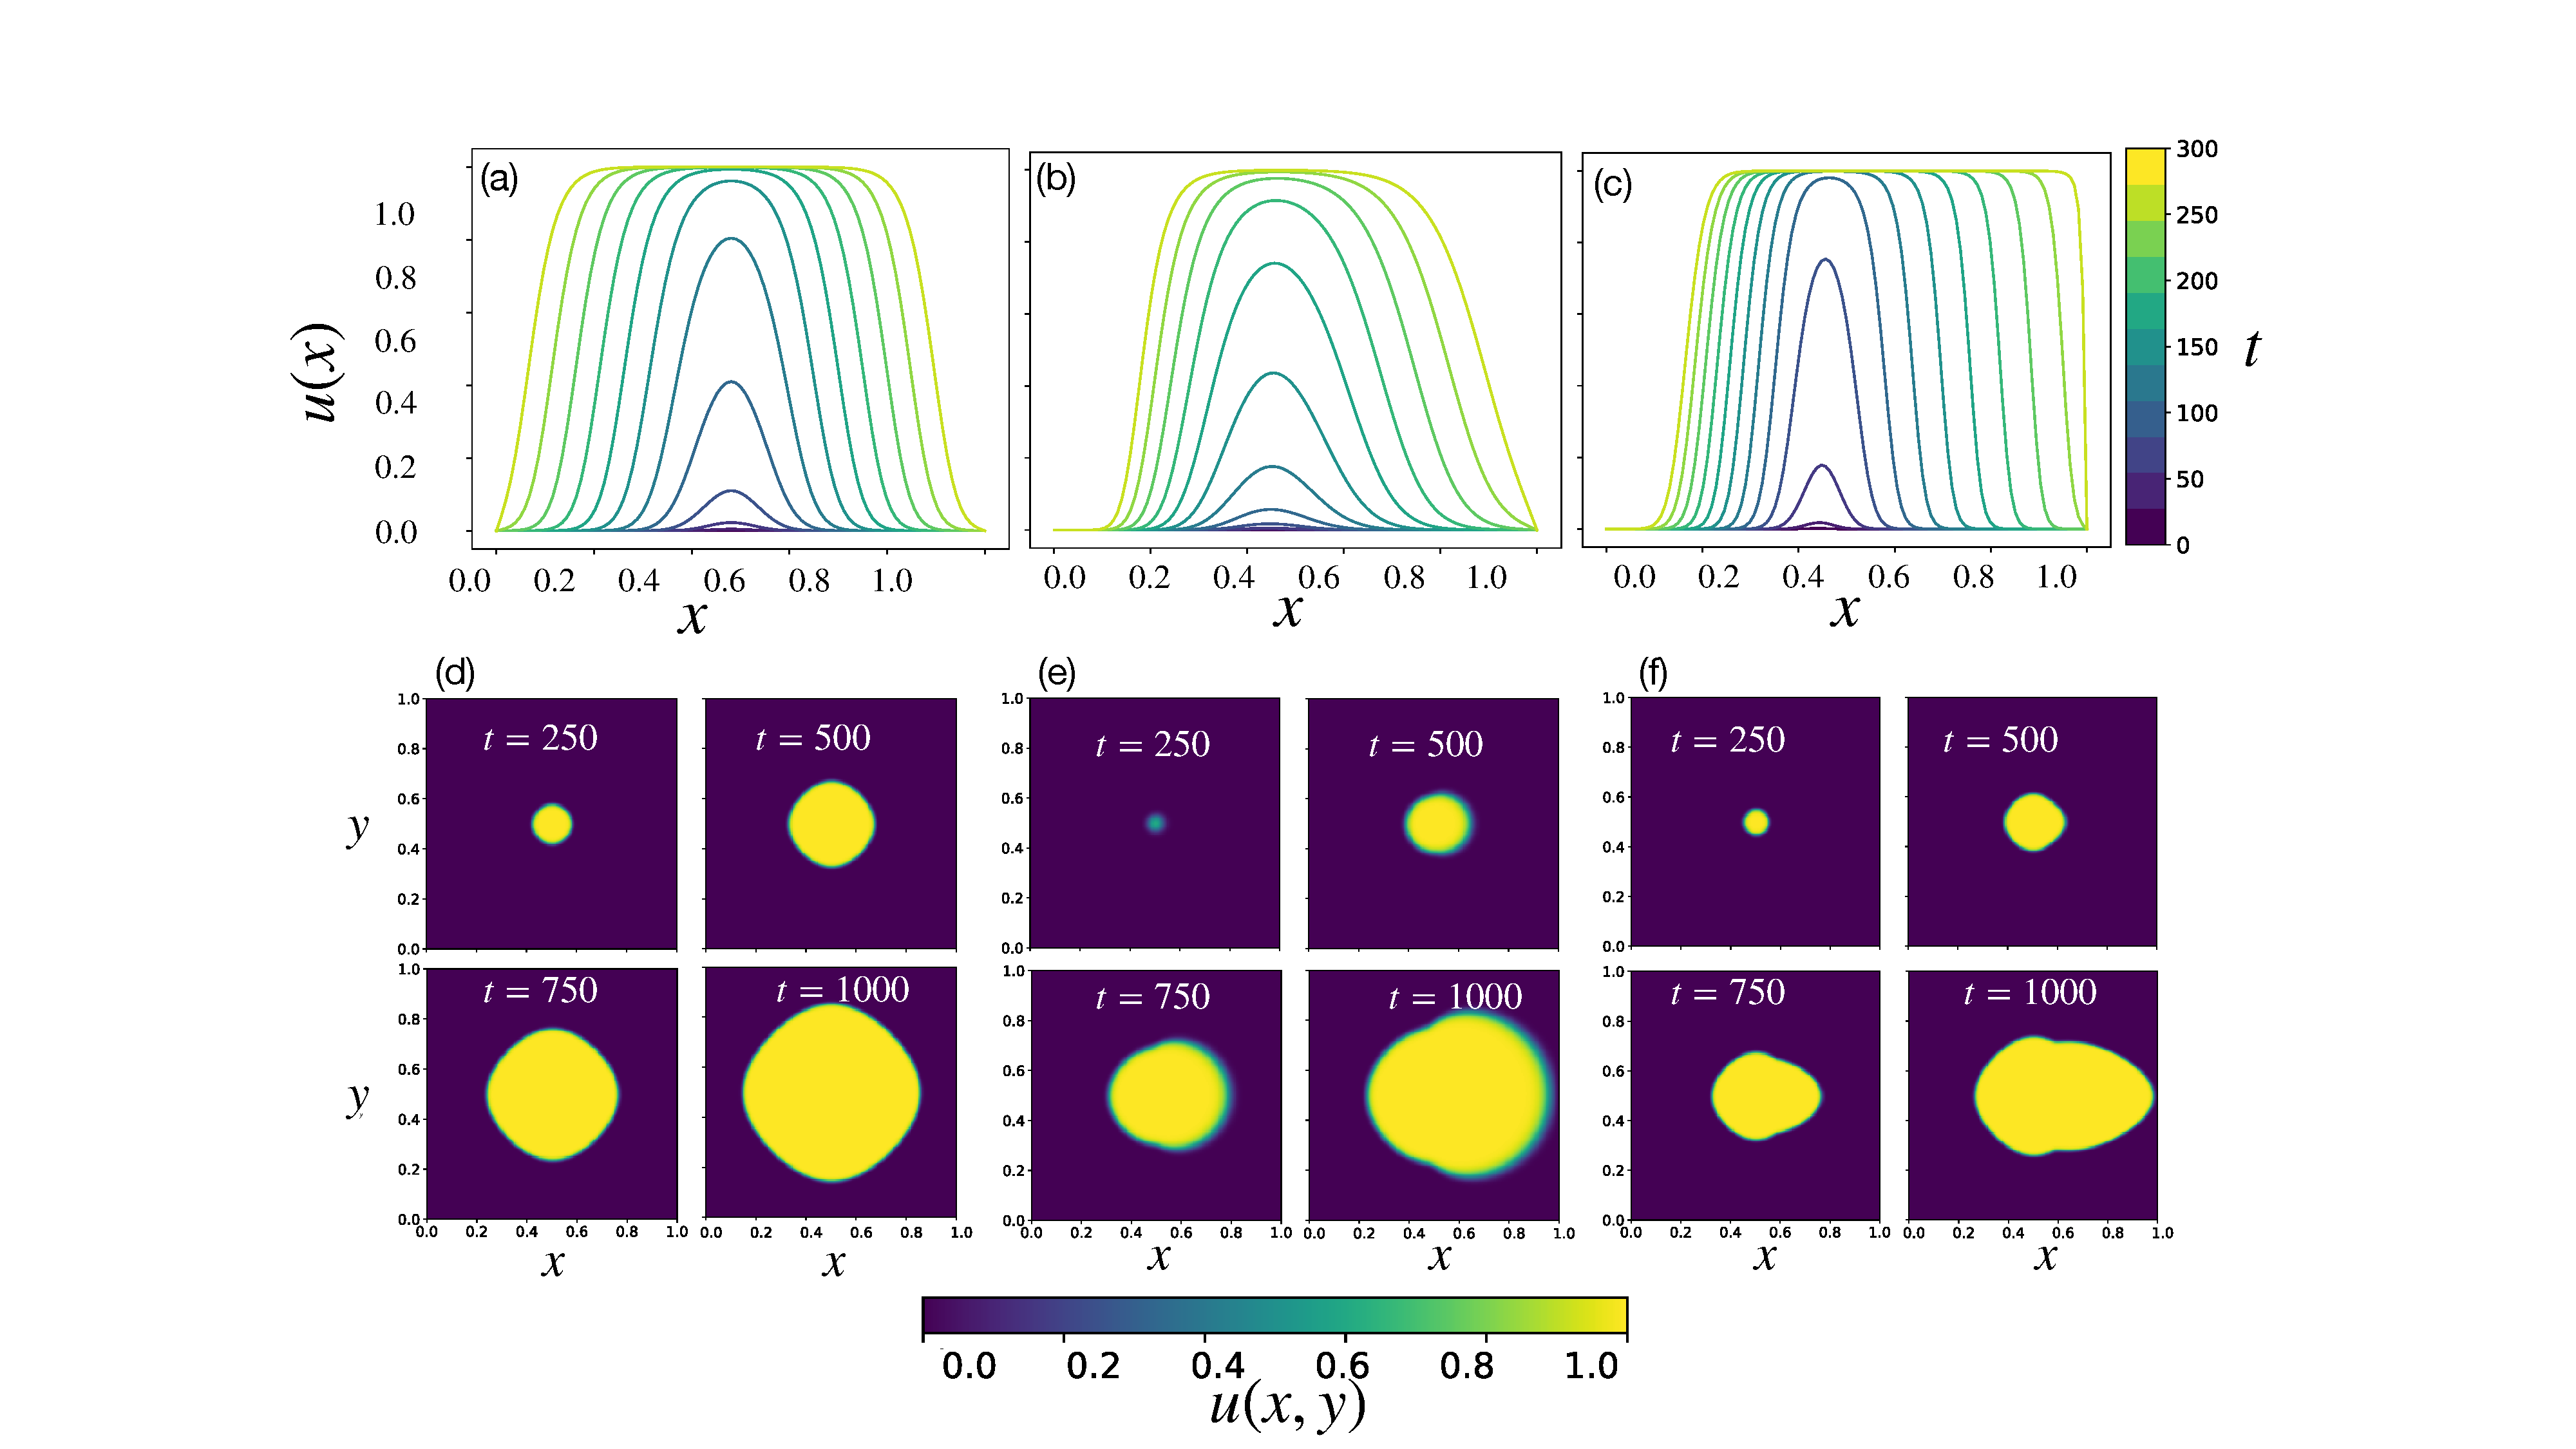
\includegraphics[scale=0.325]{chapter2/figures/FKPP.pdf}
    \caption{
    Simulating the FKPP model in one and two spatial dimensions with parameters $r=0.10$, $\mathcal{D}=0.10$, and $K=0.00$. 
    In all panels, a non-zero field value is initialised at the domains mid-point (i.e. $u(0.50)=0.10$) at time $t=0$.
    Then, simulations evolve according to a forward time centered difference (FTCD) finite difference scheme and
    follow dirichlet boundary conditions. 
    (a) Symmetric growth and diffusion in $1D$.
    (b) An asymmetric diffusion-gradient increasing from left to right in $1D$.
    (c) An asymmetric growth-gradient increasing from left to right in $1D$.
    (d) Symmetric growth and diffusion in $2D$.
    (e) An asymmetric diffusion-gradient increasing from left to right in $2D$.
    (f) An asymmetric growth-gradient increasing from left to right in $2D$.}
    \label{fig:fkpp}
\end{figure}

From these conditions, we can see that $\mathcal{D}$ and $r$ control the thickness of the wavefront,
which can be inferred by the quantity  $\ell_{w} \sim \sqrt{ \frac{\mathcal{D}}{r}}$ 
(as can be seen by the cancellation of units, i.e. $\frac{length^2}{t} \frac{1}{t^{-1}}$).
For a large $\mathcal{D}$ and small $r$, the wave-front extends over a larger region, as 
demonstrated in Figures \ref{fig:fkpp}(b) and (e). Conversely, for
small $\mathcal{D}$ and large $r$, we have a thin wavefront, shown in Figures \ref{fig:fkpp}(c) and (f).
For all panels shown in Figure \ref{fig:fkpp}, the travelling front speed remains
approximately constant that can be understood through the predicted front velocity:
\begin{equation}
    \label{eq:fkpp_vel}
    v \geq v_{min} = 2\sqrt{r\mathcal{D}}
\end{equation}
where $v_{min}$ is the minimum wave-speed admitted by the front\footnote{
The reader can find comprehensive derivation in \cite{murray2002mathematicalbiology}, 
in Chapter 11 "Biological Waves". In there, we see that strictly speaking Equation \ref{eq:fkpp_vel} 
is incorrect in two spatial dimensions on account of wavefront curvature. However, it still provides
a reasonable estimate.}.
The numerical stability of simulations is ensured provided that the Courant–Friedrichs–Lewy (CFL) condition
is met \cite{cfl-condition}.
In the case of the FKPP model, the CFL condition is given by: $\mathcal{D} \times (dt/dx^2 )< \frac{1}{2}$
where $dx$ and $dt$ represent the discretized domain and time-steps respectively.

The travelling-wave behaviour of Equation \ref{eq:fkpp} has been used in various epidemiological applications
\cite{britton1986reaction, murray2002mathematicalbiology, klein2010reaction,bianco2013reaction, yano2017kinetic}.
Indeed, the FKKP model has close connections to alternative travelling-wave models examined in the context of
plant epidemics \cite{heesterbeek1987modelling, van1988focus}. In the context of plant disease models, 
these travelling waves generally emerge from the inclusion of short-range exponentially-bounded\footnote{
Here, the choice of exponential distribution can be considered as slightly longer-range than a Gaussian dispersal kernel 
with the same scale parameter. Although, both kernels are still fundamentally thin-tailed.} dispersal contacts
between individuals\textemdash as proved theoretically by \cite{mollison1977spatial} who compared the FKPP model against 
exponentially-bounded `contact' models.

At first glance, the reaction diffusion (\acrshort{rd}) FKPP travelling wave presents a simple, 
intuitive place to begin modelling the spread of disease through a population of trees.
However, following earlier work on turbulent diffusion \cite{scherm1996velocity},
epidemic systems that spread through fat-tailed LDD are now thought to exhibit an accelerating `dispersive' 
wavefront \cite{pybus2012unifying, cowger2005velocity},
in contrast to the constancy predicted by Equation \ref{eq:fkpp_vel}. In this case,
dispersal becomes evermore efficient as the disease front extends over larger areas.

\begin{figure}
    \centering
    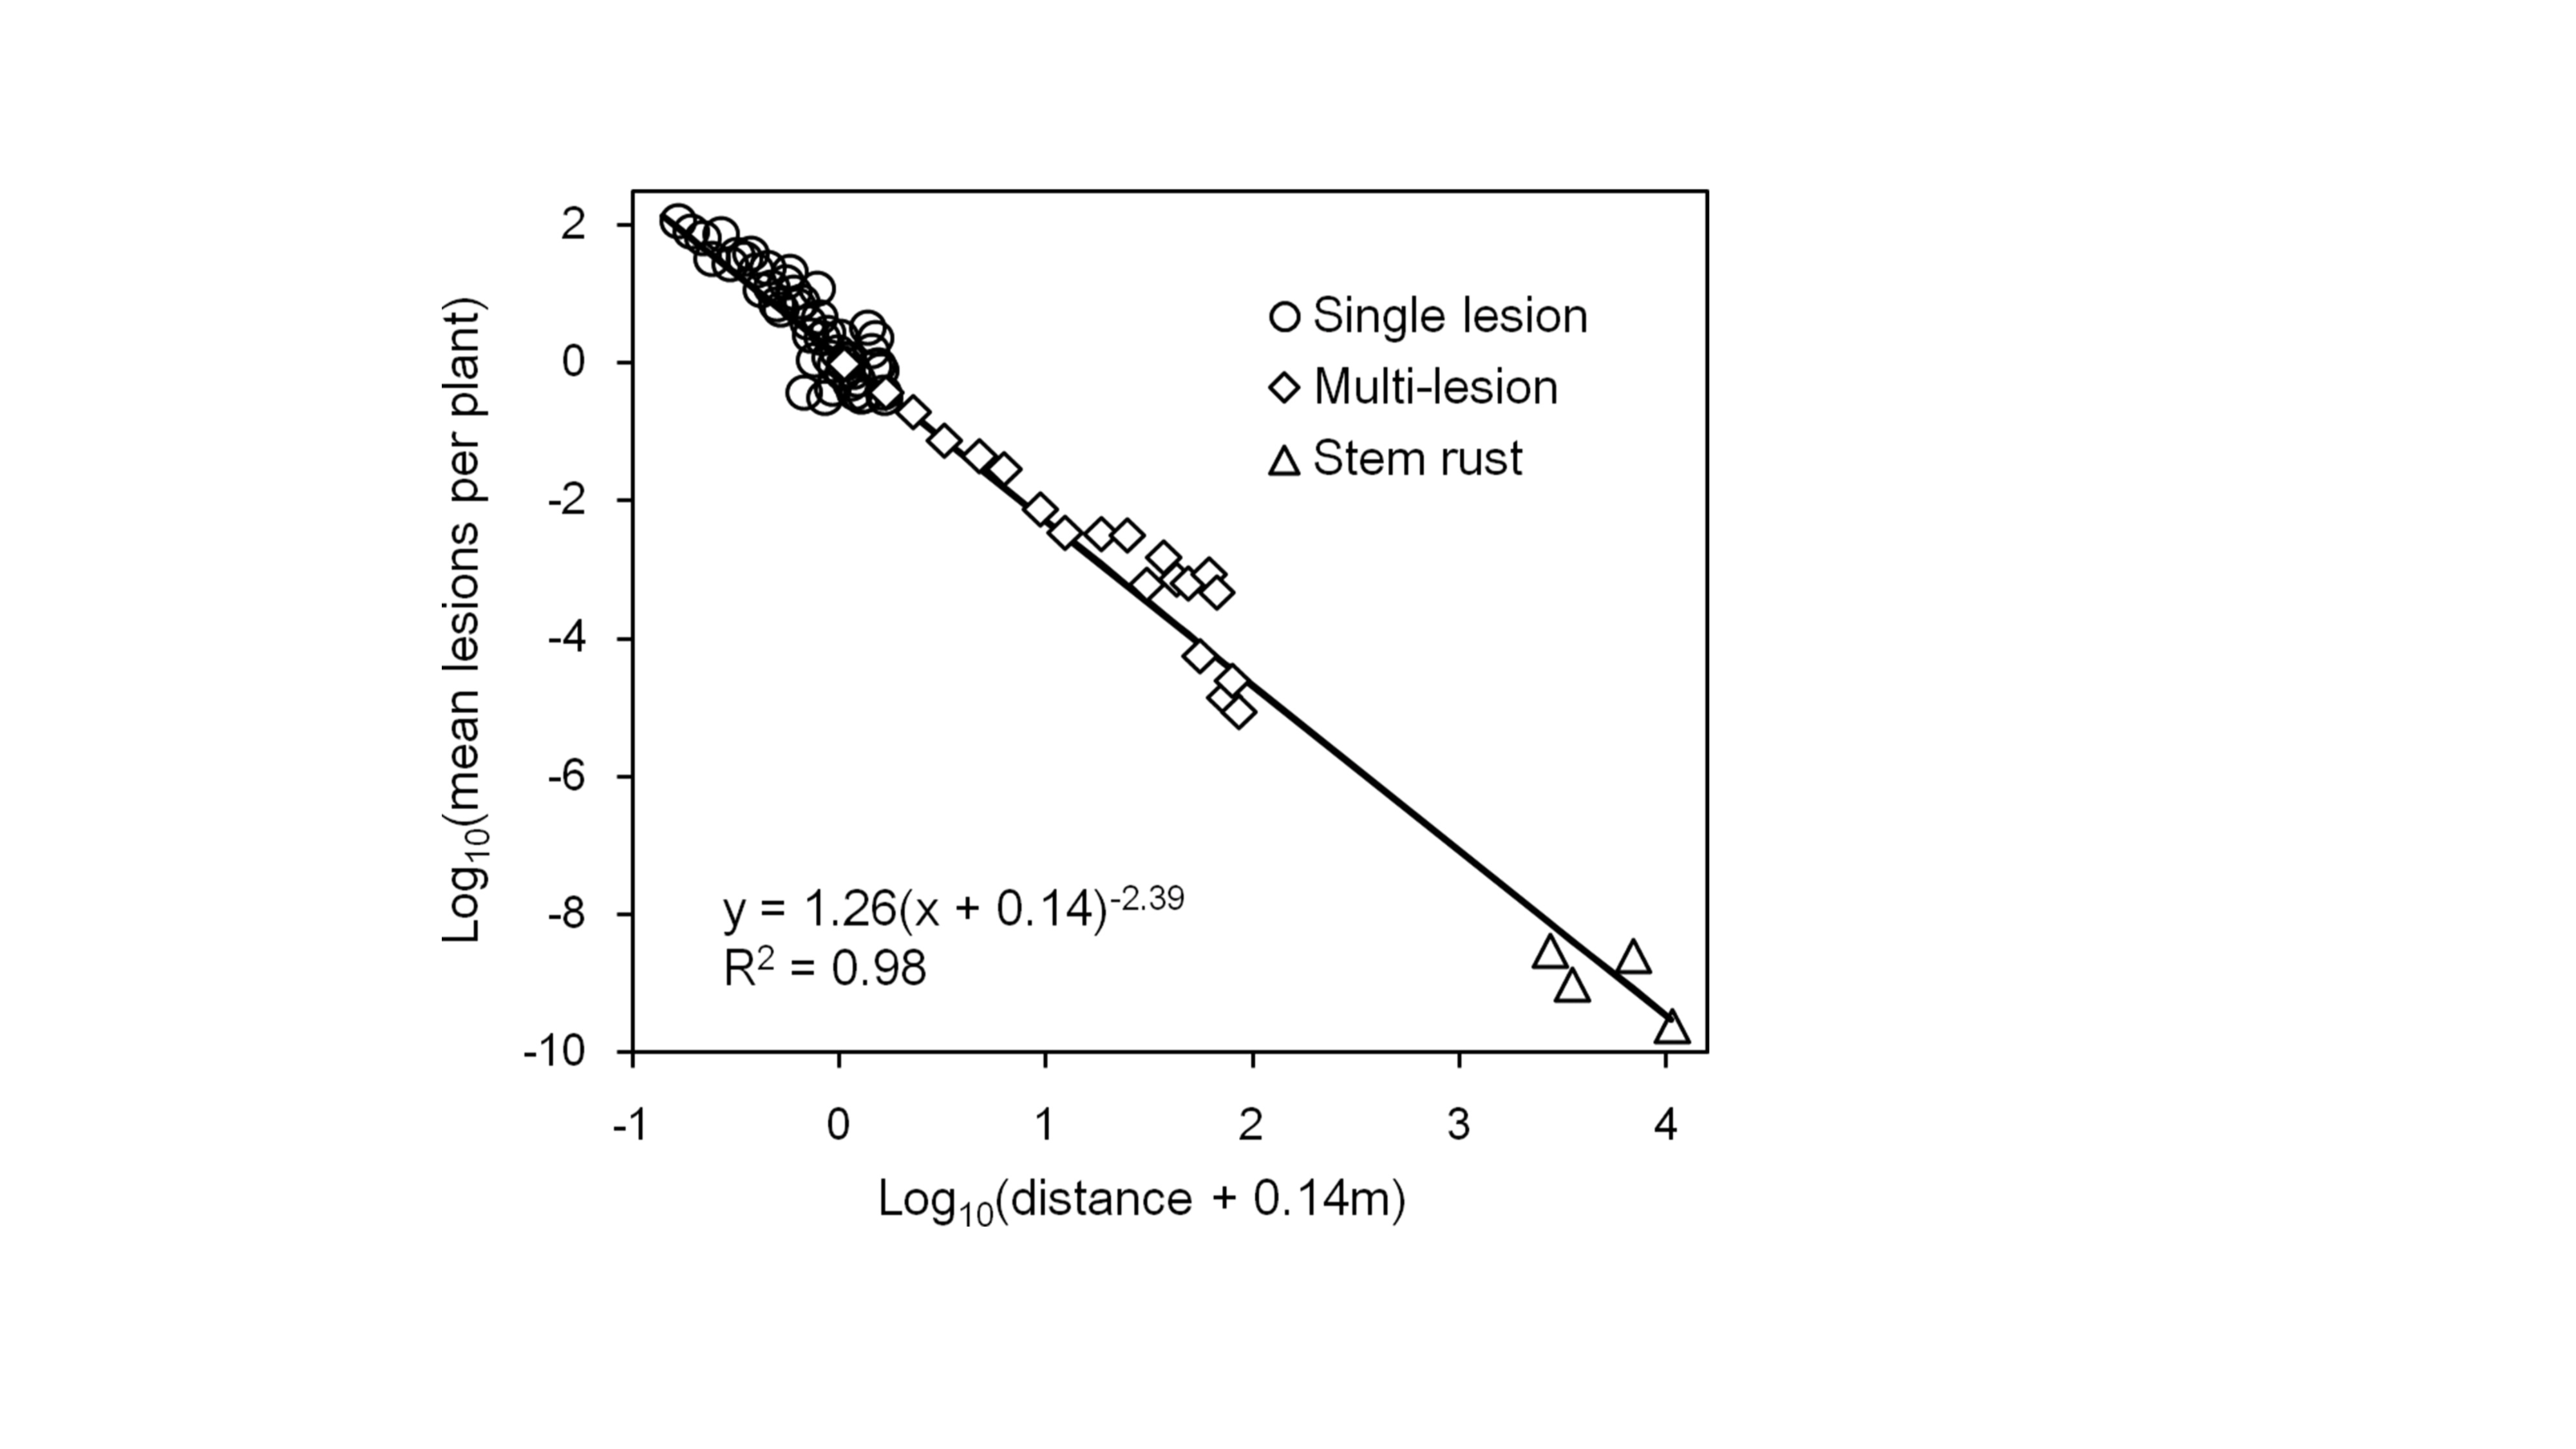
\includegraphics[scale=0.3]{chapter2/figures/multi-spread.pdf}
    \caption{Wheat strip rust prevalence with distance shown for three data sources, as displayed in \cite{severns2019consequences}.
             The authors collated data from different wheat strip rust studies and found that disease prevalence 
             over different spatial scales could all be fitted to a common power law\textemdash shown in the bottom left corner. 
    }
    \label{fig:WSR-prevelance}
\end{figure}

Inverse power law dispersal kernels are thought to be of significant importance with accelerating disease
fronts, following from their fat-tailed leptokurtic nature and subsequent scale-invariance. In particular,
they have been successfully used to fit spore dispersal data over five orders of magnitude \cite{mundt2009long}, 
from $20\mathrm{m}$ to continental spatial scales.
Power law scale invariance was examined by \cite{severns2019consequences} for wheat strip rust (\acrshort{wsr}) epidemics. 
In particular, the authors constructed wheat plantations and artificially introduced WSR to measure its prevalence over time. 
Consequently, the spatio-temporal WSR incidence rates strongly supported
an accelerating, disperseive, wavefront. 

In addition to dispersive waves, \cite{severns2019consequences} aggregated other WSR prevalence studies over different spatial 
scales and fitted the combined data to one common inverse power law ($y=a(x+c)^{-b}$), shown in Figure \ref{fig:WSR-prevelance}.
Generally, we see that WSR induces less lesions with distance, and that infections can arise up to $10\mathrm{km}$ away from the source,
illustrated by triangles in the lower right hand corner.
An exponent of $b=2.39$ provided a good fit for all scales, suggesting that inverse \textit{square} power laws may 
prove a useful rule of thumb to predict disease prevalence over different scales.

\section{Tree distribution datasets in Great Britain}
\label{ch2:hostdata}

Large-scale epidemic models of tree disease rest on robust, high-quality host data.
Data-driven approaches are crucial for predicting disease spread over country-wide scales, 
though collecting high-quality host data involves myriad challenges. 
Most notably, large-scale species distributions require vast datasets that demand significant economic resources
and person-hours to assemble and maintain over time. 
However, satellite-based remote sensing technologies pose an attractive solution\textemdash see \cite{camarretta2020monitoring} for a recent review of remote sensing technologies.
Despite the significant advances of remote sensing technologies, most freely available data sets still rely on traditional surveying methods to collect data throughout Great Britain (GB).
Consequently, the most widely known and widely used datasets are reviewed below.
Following this, statistically-generated species distribution models, typically based on surveyed data, are reviewed.

\subsection{National Surveys}
\label{sec:nationa-surveyes}

Surveyed data predominantly describes either: abundance, presence-only, presence-absence data. 
Generally, abundance data describes percentage canopy cover per $\mathrm{km^2}$.
In contrast, binary-valued presence-only and presence-absence data simply record if a species is present or present and absent, respectively.
Abundance captures significantly more information than presence-only data, yet unfortunately, they are in short supply.

\subsubsection{Countryside Survey}

The countryside survey (\acrshort{cs}) is a long-running, national survey of diversity and species abundance in GB \cite{wood2017long}.
The UK Centre of Ecology and Hydrology (UKCEH) undertakes the surveys, primarily funded by the Natural Environmental Research Council alongside other government agencies.
Individual surveys have been undertaken in: $1978$, $1990$, $1998$, $2007$, and $2019$. 
Random stratified sampling captures a representative species abundance\footnote{
A useful (unpublished) project merged abundance data from CS with myForest. The abundance data can be found at the Oxford University research archive: \nolinkurl{https://ora.ox.ac.uk}.} 
over of all land cover compositions, e.g. lowland acid grassland, freshwater, and broad-leaf forest.

Abundance data is collected for numerous dominant species, including trees, shrubs, ground flora and soil type, 
making the scope of CS data vast. Moreover, long-running records spanning decades reveal ecosystem trends imperative for ecological monitoring.
More recently, $100$ $1\mathrm{km^2}$ plots of vegetation and soil data were collected\footnote{
The data is free to download on the UKCEH website: \nolinkurl{https://catalogue.ceh.ac.uk}} \cite{10.5285/fd6ae272-aeb5-4573-8e8a-7ccfae64f506}.
The dataset constitutes the first of five planned surveys, part of a rolling monitoring strategy collected every five years.

\subsubsection{National Forest Inventory}

The National Forest Inventory (\acrshort{nfi}) collects and maintains forest and woodlands data in GB.
Originally, the NFI was established to help restore and expand Britain's woodlands following the First World War \cite{james1990history}.
Regular programs ($10$-$15\mathrm{year}$ intervals) implement surveys of woodland and forest size, distribution, composition and condition across GB.
Records cover areas over $0.5\ \mathrm{ha}$ and $20\%$ coverage.
As of $2019$, $622,381$ individual records exist, spanning $2.9 \times 10^6\ \mathrm{ha}$ over $13\%$ of the total land cover within GB.
NFI data comprise ESRI shape files\footnote{
Free to download at: \nolinkurl{https://data-forestry.opendata.arcgis.com}},
that outline numerous forest types, e.g. broadleaved, conifer, mixed-predominantly broadleaved or mixed predominantly conifer.
Despite an extensive coverage, publicly available NFI surveys describes presence-only data\textemdash with no proportion or species coverage.
Although, additional datasets are available to purchase, including: 
1) Tree species percentage per region by woodland type
2) Tree species proportions within the upper canopy of each NFI sample plot, without supplying the exact location of the individual sample plot.

\begin{figure}
    \centering
    \includegraphics[scale=0.2]{chapter2/figures/NFI-figure.pdf}
    \caption{NFI data super imposed onto a Google earth image, taken from a report (unpublished) by S. Orozco-Fuentes et al.
             NFI data covering Thetford Forest Park ($16.684 \mathrm{km}^2$) is shown as a polygon in the NFI `woodland' category.
             Data is interpreted as the conifer forest type. Here, surveys comprises presence-only data, and no tree species percentage cover
             is reported. NFI data extends throughout $\sim 13\%$ of land coverage in GB and large non-woodland areas remain un-surveyed.}
    \label{fig:NFI-data}
\end{figure}

\begin{figure}
    \centering
    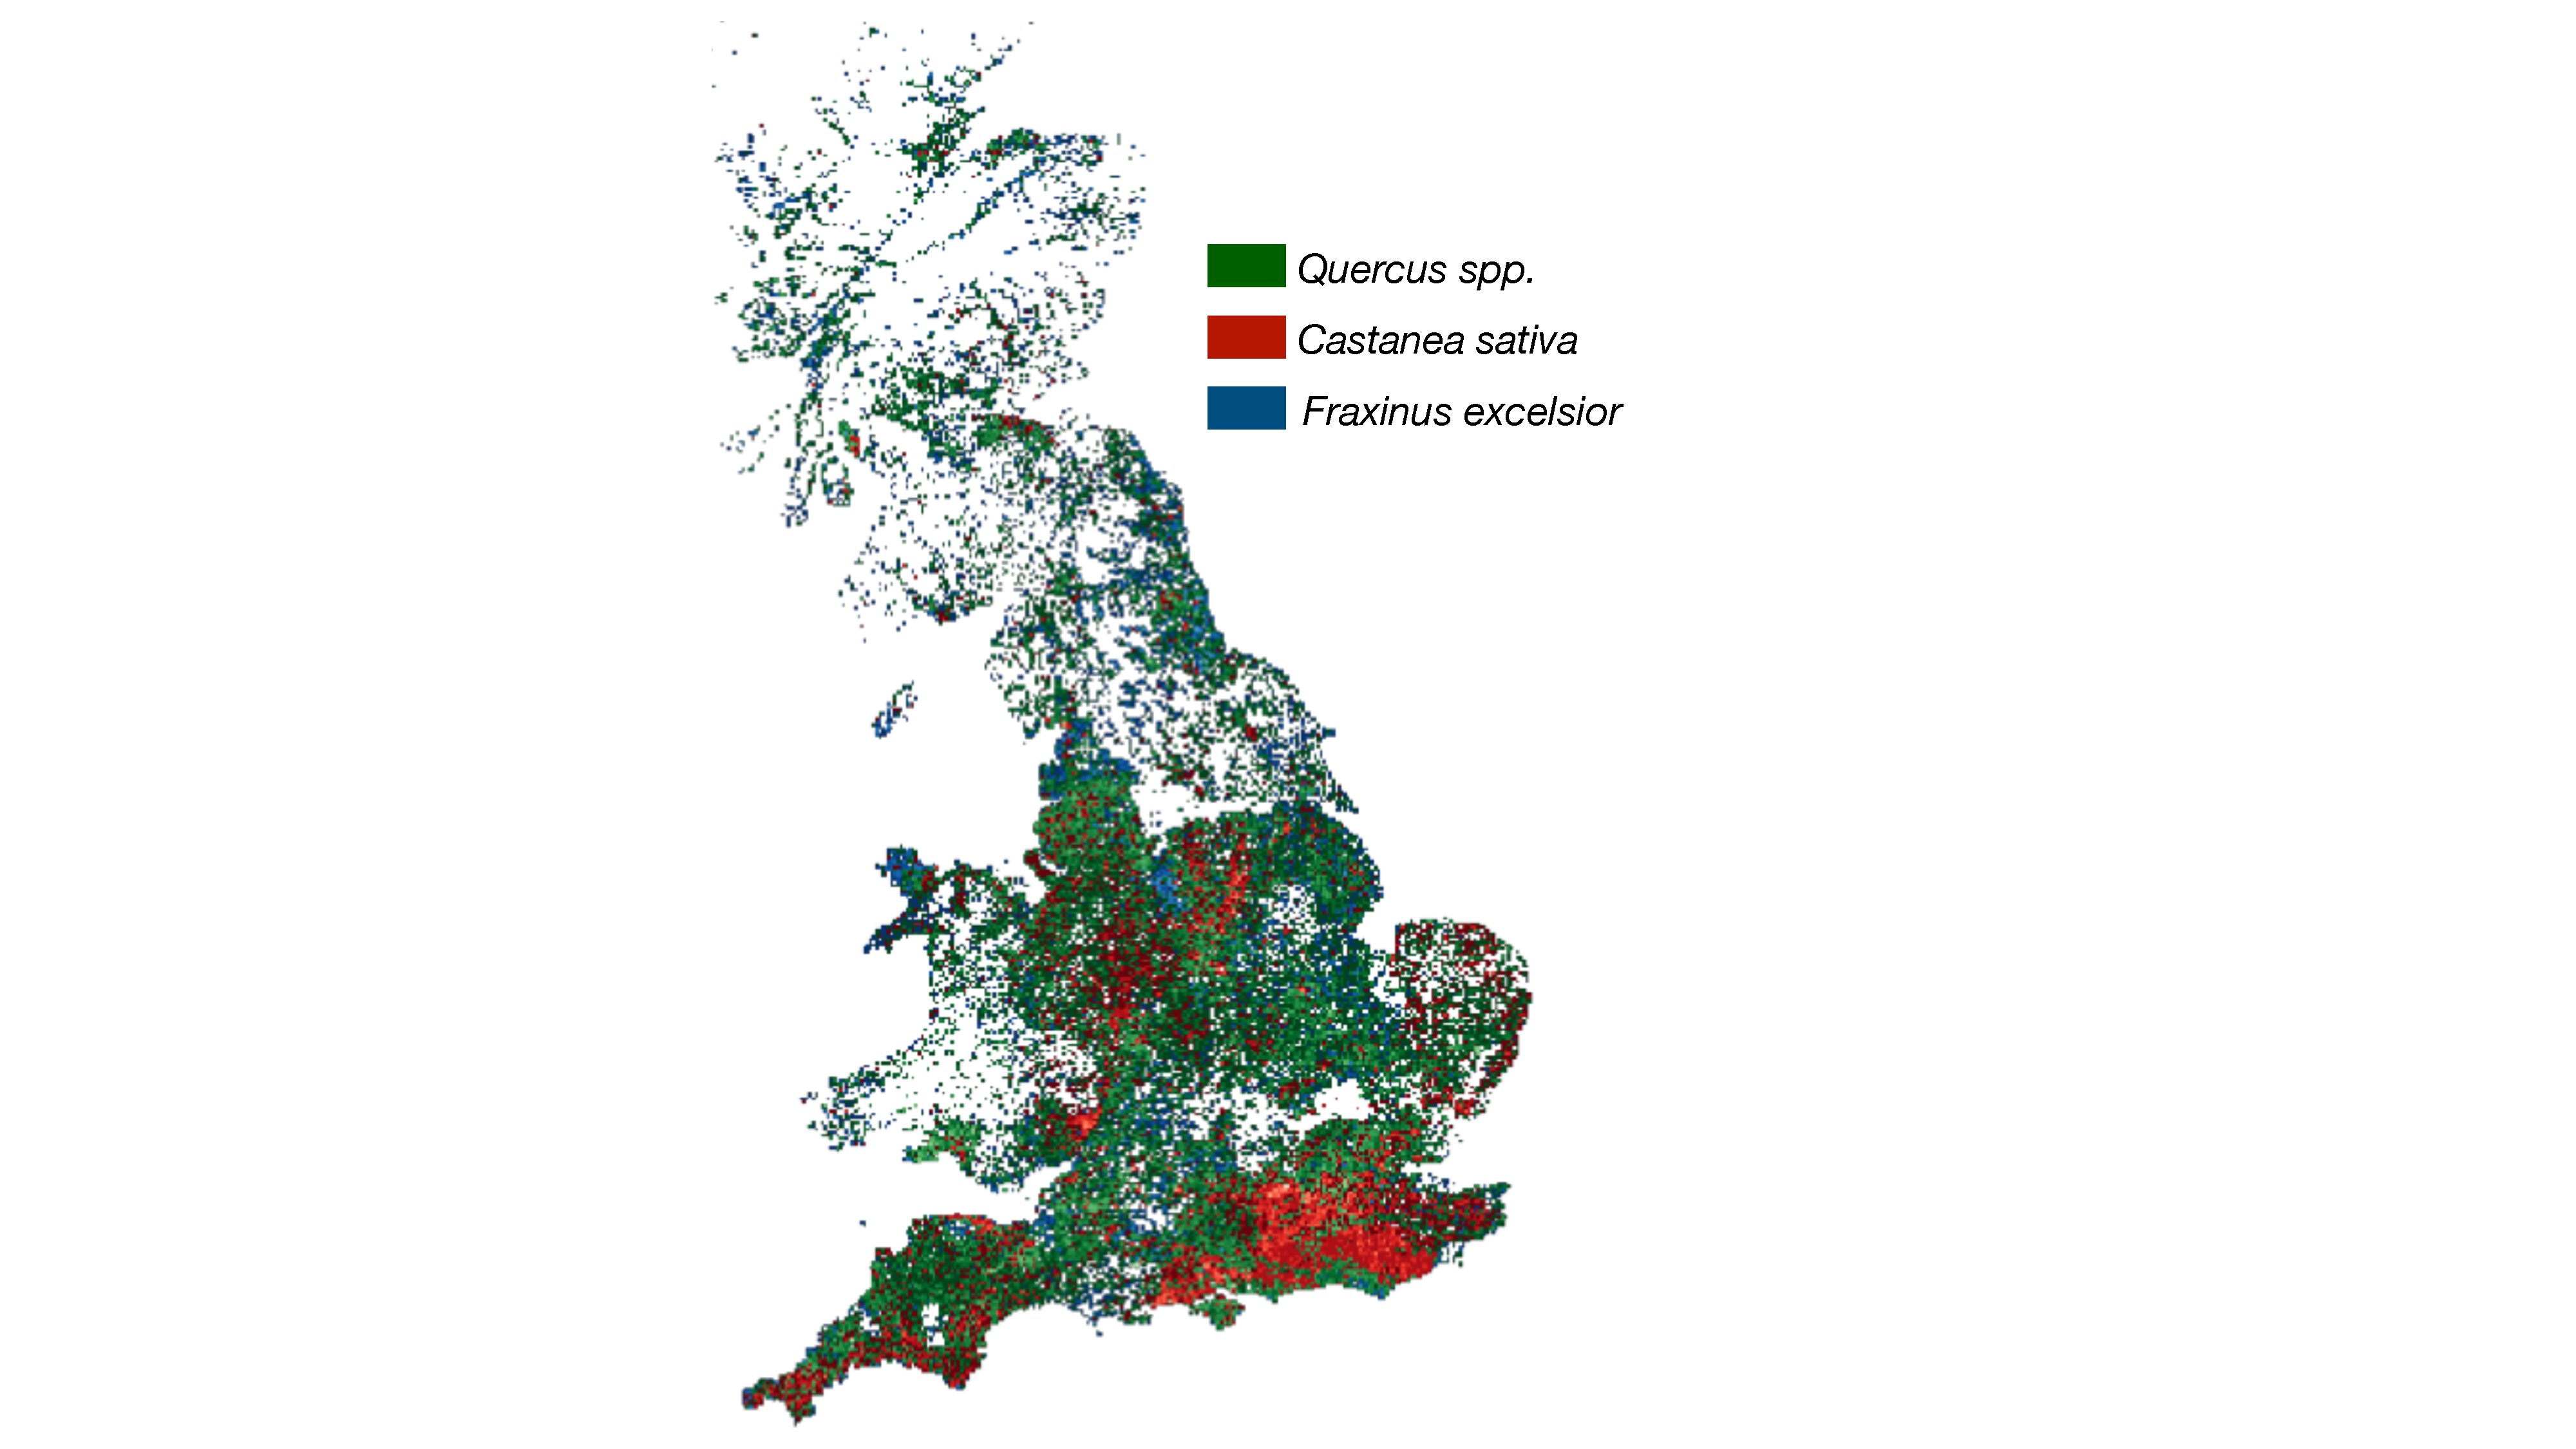
\includegraphics[scale=0.25]{chapter2/figures/bsbi-data.pdf}
    \caption{BSBI presence-only datasets\textemdash as reconstructed by S. Orozco-Fuentes et al. (unpublished).
    Three important large deciduous tree species, European ash (\textit{Fraxinus excelsior}), 
    Oak (\textit{Quercus spp.}), and sweet chestnut (Castanea sativa), are overlaid onto the same map at $\mathrm{2km \times 2km}$ resolution.
    The BSBI datasets are extensive and report presence-only data over a country-wide scale.
    }
    \label{fig:bsbi-data}
\end{figure}

\subsubsection{Botanical Society of Britain and Ireland}

The Botanical Society of Britain and Ireland (\acrshort{bsbi}) has recorded species presence-only data since $1950$.
BSBI datasets are publicly available\footnote{BSBI data can be downloaded from: \nolinkurl{https://database.bsbi.org}.} upto a
resolution of $\mathrm{2 km \times 2km}$, though records upto $\mathrm{100 m \times 100 m}$ are available to registered members.
As of $2020$, BSBI records are collected at $\mathrm{1 km \times 1km}$ square resolution or better\textemdash making the datasets among the 
highest-resolution surveys collected by traditional methods. The BSBI distribution database contains records of plants and charophytes
as reported by users and conservationists with MapMate\footnote{MapMate is software designed to aid users to share ecological data: \nolinkurl{https://www.mapmate.co.uk}}.
Despite the availability of high-resolution data, observations are collected ad hoc by users and not curated scientifically.
Moreover, the distributions contain both well-surveyed and poorly-surveyed plots of land likely to carry uncertainties.
As such, BSIBI data is helpful to reconstruct several baseline tree distributions across GB, as demonstrated by \cite{hill.data}.

\subsection{Species distribution models}

In the absence of extensive host data, species distribution models (\acrshort{sdm}s) aim to generate synthetic data, typically from less-extensive surveys.
SDMs were first developed in the $1990$s, and have subsequently become fundamental to ecological and biogeographical inference studies.
Synthetic distributions have been used to examine biodiversity, conservation, resource management, 
ecology and climate change \cite{franklin2013species, skov2016real, wittmann2016confronting, 10.3958/059.037.0110, zhang2019using}.
The vast majority of SDMs fall into two categories: correlative \cite{srivastava2019species}, and mechanistic \cite{shabani2016comparison}.

Correlative SDMs relate (widely available) presence-only, or presence-absence, data to several environmental predictor variable datasets.
For tree species, predictor variables include temperature, precipitation, altitude, and soil type \cite{ray2021multi, hill.data}.
Following this, a species distribution map can be predicted, albeit with  uncertainties and errors.
Commonly used statistical methods include Regression 
(i.e. General Linear Models, General Additive Models, Multivariate Adaptive Regression Splines) and Machine Learning
(i.e. Artificial Neural Networks, Classification And Regression Tree, Random Forest). 
The general correlative approach is reflected in Figure \ref{fig:sdm}; for a more in-depth review of correlative SDMs, see \cite{SDM_1}.

Correlative SDM approaches require little to no prior knowledge of the physiological processes that link organism and environment.
Hence, mechanistic methods aim to incorporate an organisms behavioural, physiological, and morphological constraints to the environment, 
as reviewed by \cite{kearney2009mechanistic}. However, linking a species physiological response to the environment comes with significant
computational challenges, as it typically relies on vast, multi-variable time-series datasets \cite{shabani2016comparison}.

\begin{figure}
    \centering
    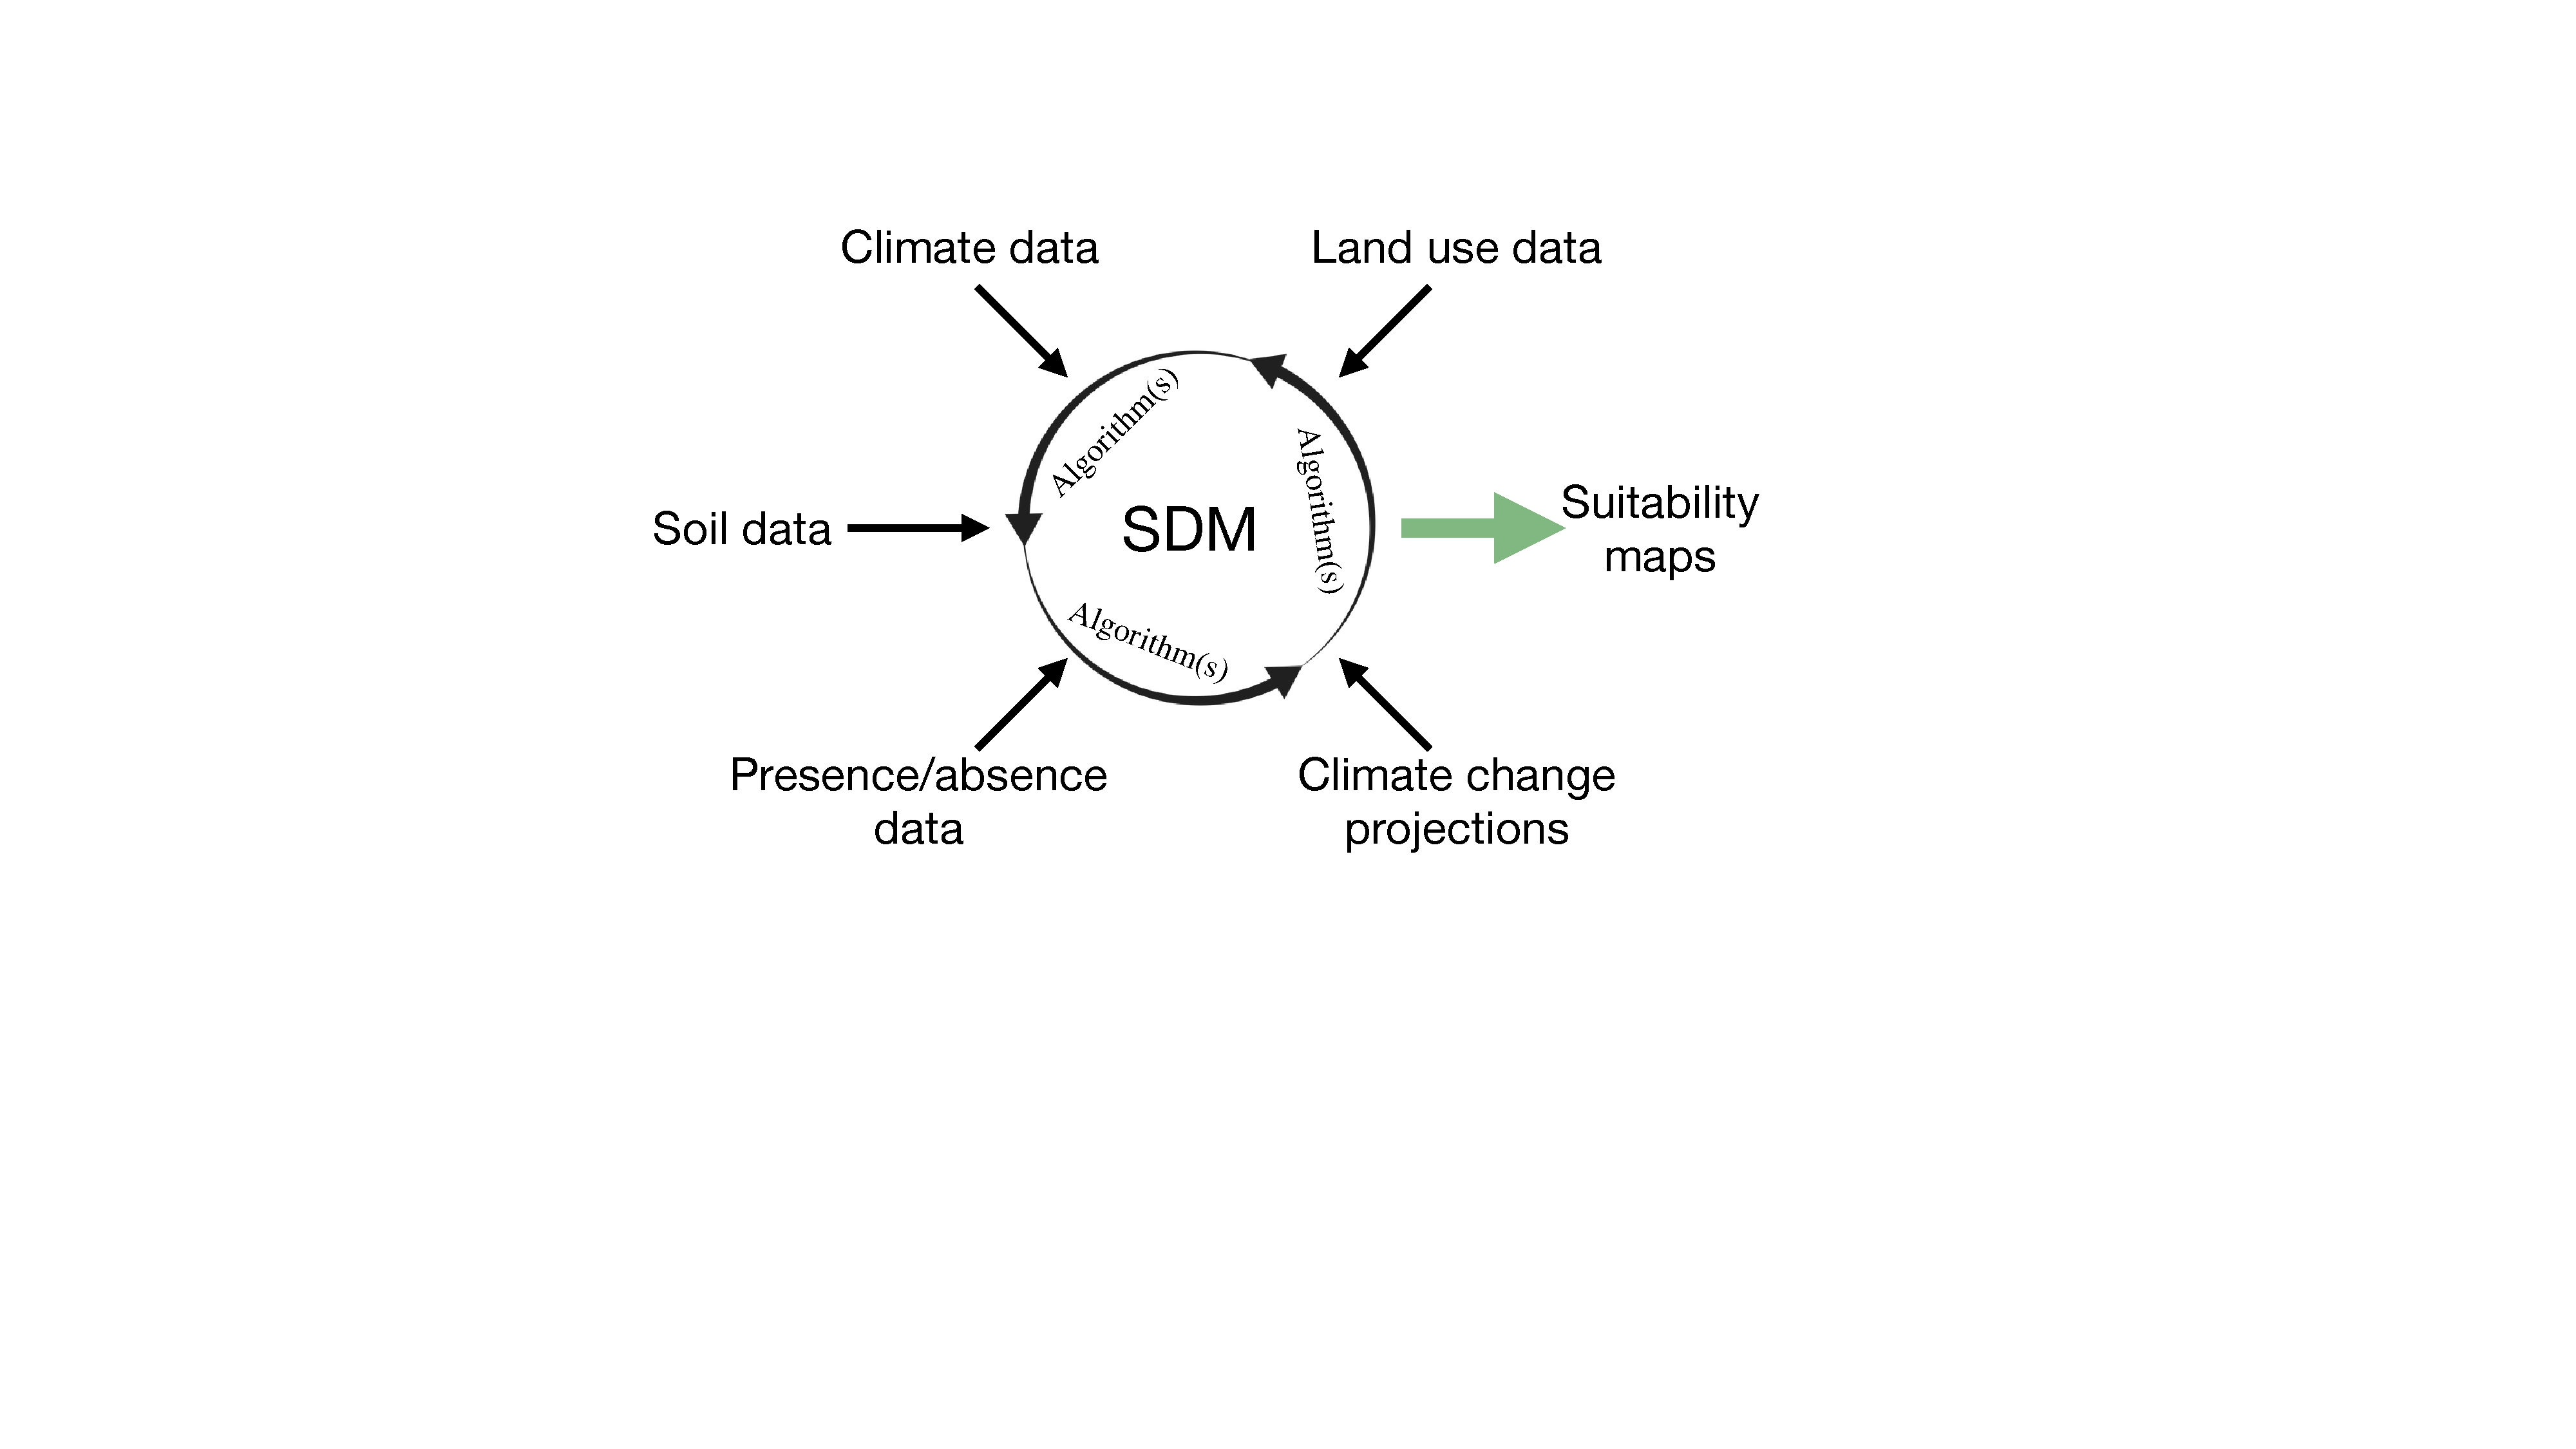
\includegraphics[scale=0.35]{chapter2/figures/SDM-fig.pdf}
    \caption{A graphical species distribution model (SDM) illustration, adapted from \cite{SDM_1}. 
             A variety of predictor variables and input data sources are used in conjugation with modelling algorithms to produce
             a habitat suitability map.}
    \label{fig:sdm}
\end{figure}

A review paper by \cite{guillera2015my}, revealed a diverse use of SDMs.
Out of $100$ publications reviewed by \cite{guillera2015my}, SDMs were applied to: 
1) managing threatened species ($16\% $ of articles) 
2) predicting climate change impacts ($13\%$) 
3) understanding phylogeographic patterns ($9\%$) 
4) controlling threatening processes ($8\%$) 
5) landscape management ($8\%$) 
6) biological invasions ($7\%$). However, no epidemic applications were reported.

Nevertheless, a thorough literature search revealed a variety of epidemiological SDM applications.
The crossover between ecological SDM methods and epidemiology has been referred to as `Infectious Disease Cartography' \cite{KRAEMER201619}.
With Infectious Disease Cartography, one seeks to map the likelihood, or risk, of infectious disease outbreaks and produce risk-maps.
A number of publications have applied SDMs livestock diseases \cite{hollings2017species}, and human-based diseases including the global 
distribution of Dengue Fervour \cite{bhatt2013global} and Zika virus \cite{messina2016mapping}, and Anthrax in Kenya \cite{otieno2021modeling}.
However, SDM applications for tree disease epidemics appear absent from the literature.

\subsubsection{Predicting tree abundance}

SDM-generated tree occurrence data have limited applications to ecologists and forest managers.
This motivates statistically-generated abundance data that includes significantly 
more information about the population occupation/density and ecosystem.
Modellers have examined numerous approaches to predict species abundance;
including, linking the abundance-occupancy relationship \cite{gaston2000abundance} and
the scaling pattern of species occupancy over progressively smaller spatial scales \cite{hui2009extrapolating}.

An interesting, and highly relevant, approach to predict the abundance of common tree species in Great Britain was put forward by \cite{hill.data}.
At a high level, BSBI presence-only data were combined with a series of environmental covariates using a species distribution model to 
produce a map of predicted occurrence data. Then, random forest regression was employed with a training sample ($70\%$) of less extensive abundance 
data (consisting of CS, myForest and Bluesky's National Canopy Map). 
Results were then cross-validated with the remaining ($30\%$) abundance data; Figure \ref{fig:hill-method} displays a
flow-diagram of the method presented by \cite{hill.data}. 

A more detailed explanation of the treatment proposed by \cite{hill.data} follows:
\textbf{Stage 1)}
\textit{
\begin{itemize}
    \item Presence-only BSBI data was downloaded for $25$ common species of trees in GB, 
    and all records less than $\mathrm{2km \times 2km}$ resolution were discarded.
    Next, the presence-only data was converted into presence-absence data by considering
    `well-surveyed' records that Hill et.al defined as having a minimum of two survey
    between $1950$ and consisting of $50$ species. Species missing from these 
    well-surveyed areas were assumed truly absent. 
    \item Using biomod2 \cite{thuiller2016package}, a SDM was then fitted against a cohort of 15 environmental variables, e.g.
    soil type (European Soil Database), temperature (Worldclim), precipitation (Worldclim), altitude (Worldclim),
    type of land cover (Countryside Survey), among others. The net result was a map of predicted occupancy at $\mathrm{1 km \times 1 km}$ 
    resolution.
    \item For each species, predictions from a suit of models\textemdash GLM, GAM, CTA, GBM, RF\textemdash were
    repeated and combined into an ensemble distribution model. Each model was cross-validated against
    $30\%$ of the well-survyed BSBI presence-absence data using the receiver operator curve (\acrshort{roc}) and the true skill statistic (\acrshort{tss}).
    \cite{hill.data} then selected the best performing predicted occurrence for each species.
\end{itemize}
}
\textbf{Stage 2)}
\textit{
\begin{itemize}
    \item Abundance data from CS and myForest were both expressed as hectares covered per kilometer 
    squared ($\mathrm{ha/km^2}$). This entailed using woodland cover from the NFI dataset to multiply
    the percentage cover of each species within a woodland patch, with a proportion of woodland cover per kilometer.
    \item Random forest (RF) regression then modelled the relationships between (CS and myForest) abundance data with
    the SDM-generated map of predicted occupancy. In addition, RF regression used four covariates, 
    three of which consisted of Bluesky's National Canopy data (i.e. total tree cover, woodland tree cover, non-woodland tree cover)
    and NFI edge broadleaved woodland (i.e. within $50\mathrm{m}$ of non woodland) data.
\end{itemize}
}

The abundance datasets produced by \cite{hill.data} combine several mainstream tree datasets in GB; moreover, 
constructing the ensemble model involved a variety of statistical models.
The predicted occurrence data was examined against the ROC \cite{jimenez2012insights}.
Most species demonstrated functional ROC scores between $0.71$ and $0.96$ and performed exceptionally
well for ash ($0.96$) and oak ($0.90$).  

Although, numerous assumptions underpinned the methodology.
Primarily, the BSBI dataset used by \cite{hill.data} exists through ad-hoc user and volunteer self-reports.
Thus, some regions are more surveyed than others over the years, this led Hill et al. to make the 
`well surveyed' recorded assumption (i.e. only considering records surveyed twice since $1950$ containing a minimum of $50$ species).
The assumption permitted the conversion of raw presence-only to presence-absence, 
at the cost of overestimated absence in these regions. That is, even supposing $50$ species
are reported within a subset of the ($\mathrm{2km \times 2km}$ tetrad) record, other large regions could remain unsampled\textemdash
the authors did not appear to scrutinise this assumption sufficiently.

\begin{figure}
    \centering
    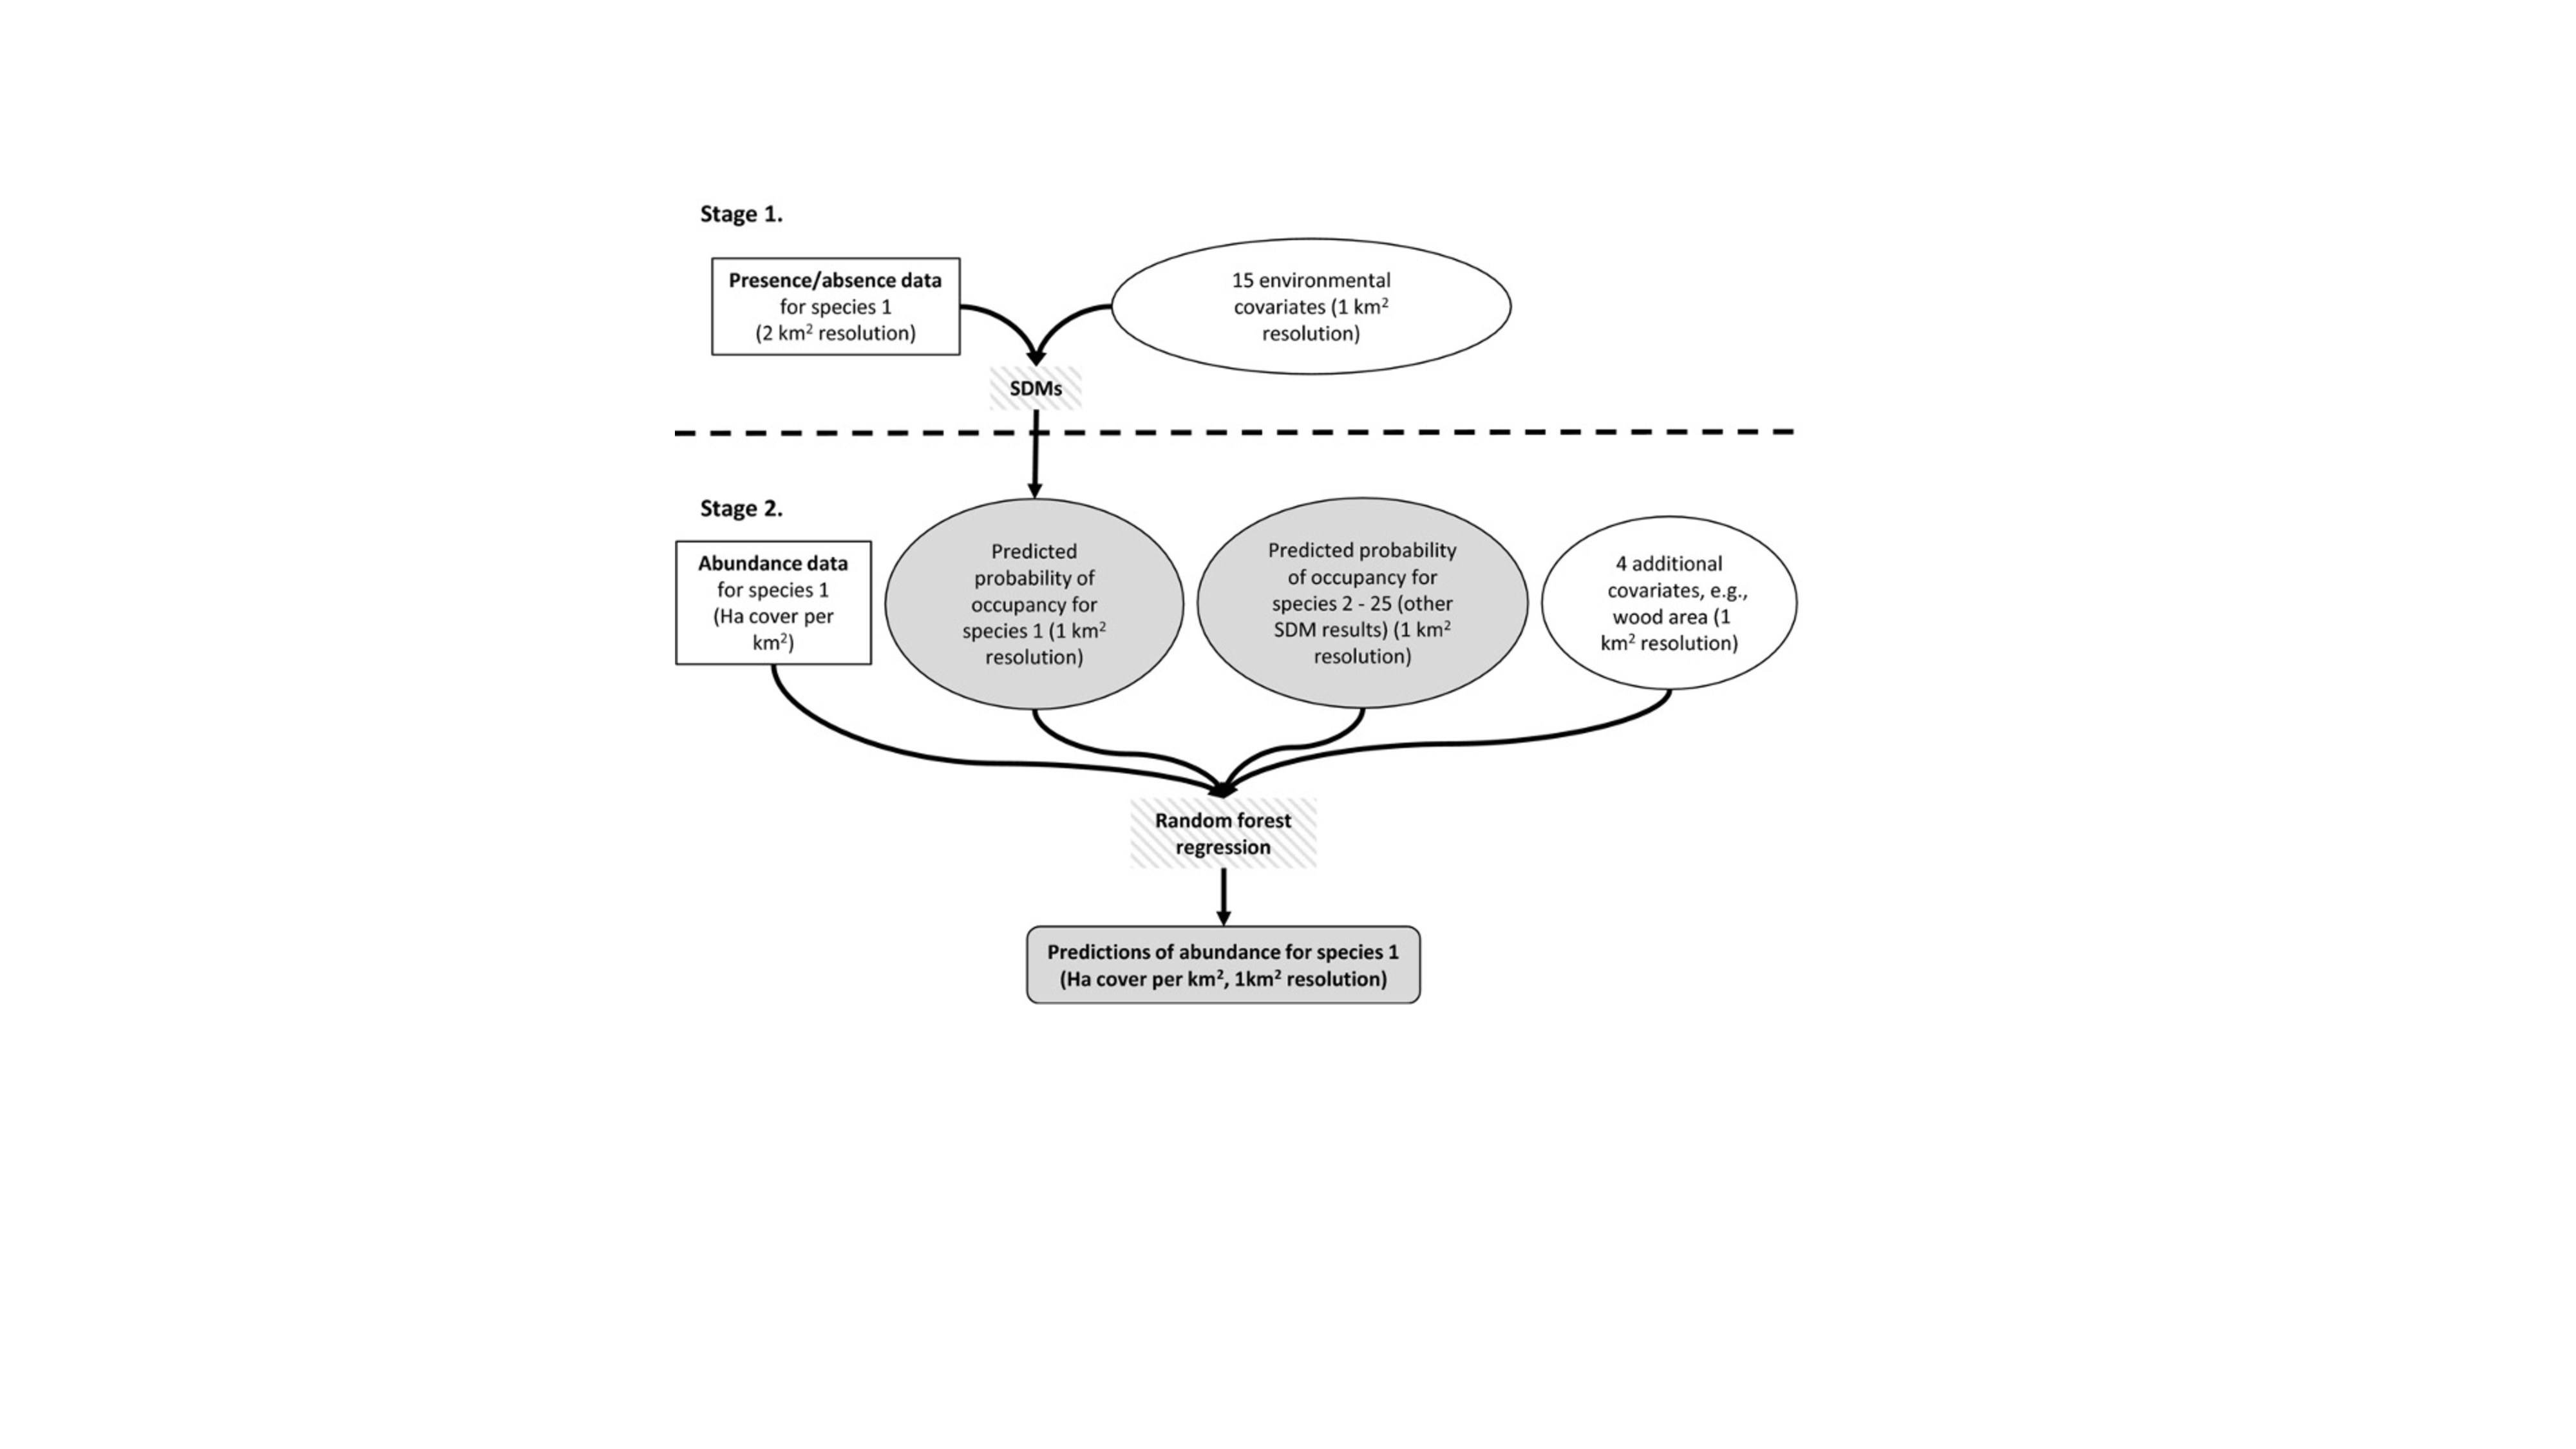
\includegraphics[scale=0.55]{chapter2/figures/hill-method-fig.pdf}
    \caption{A flow diagram of the two-stage abundance method put forward by \cite{hill.data} to model tree species abundance  
    (taken from the publications' materials and methods section).}
    \label{fig:hill-method}
\end{figure}

The RF regression used by \cite{hill.data} marked a novel approach to modelling species abundance.
The authors chose to argue in favour of RF regression because of its insensitivity toward the data distribution,
which worked well with the less comprehensive abundance data sources (as the map of abundance had a high percentage of zeros from missing records).
The abundance model quality was examined against $10$-fold validation (explained in \cite{refaeilzadeh2009cross}).
The root-mean-square error (\acrshort{rmse}), between predicted and observed abundance, generally ranged between $5$ and $10$,
where the RMSE scale reflects the response variable units ($\mathrm{ha/km^2}$), i.e. $5\%$ and $10\%$ respectively.
The result was country-wide predicted abundance.

The low amount of available abundance data in GB significantly impoverished the abundance maps produced by \cite{hill.data}. 
Consequently, datasets for the $25$ species considered will contain numerous (small-scale) errors and uncertainties. 
Nonetheless, the modelled abundance maps captured more large-scale spatial structures than the original BSBI and CS distributions.

More recently, \cite{ray2021multi} produced a similar SDM as Hill et al. for oak in GB using biomod2 \cite{thuiller2016package}.
The authors focused on mapping high-density oak woodlands (with 60$\%$ canopy cover or above) 
to predict which NFI map polygons (by forest type) were most likely to contain oak stands. 
However, \cite{ray2021multi} did not make their oak maps publicly available, nor did they produce a general-purpose
abundance map relevant for epidemiological studies. 
To date, the data sets produced by \cite{hill.data} constitute the best publicly available
country-wide maps of abundance in GB, despite their limitations.

%\item remote sensing tools were used \cite{kelly2002monitoring} to track the study of sudden oak death in California
%\item \cite{kelly2002landscape} demonstrated clustering at the landscape level, spatial structure is important

\section{Ash dieback case study}

% - the combination of ash dieback and emerald ash borer present a significant threat to UK and European ash \cite{musolin2017between}
% - managing the spread of ADB in areas already infected is hardly possible \cite{gross2014h}
% - but slowing the spread of disease is still valuable to allow ash populations vital time to recover and policy makers \cite{PAUTASSO201337}
% - multi-scale approaches have been outlined \cite{hart2020theoretical}

\label{ch2:ash-dieback}
Ash dieback presents an interesting case study of an emerging epidemic currently devastating ash
populations throughout Europe \cite{enderle2019overview}. The history and predicted evolution of ash dieback
demonstrate how an invasive, non-indigenous pathogen can spread rapidly through a foreign ecosystem that 
lacks evolutionary defences. Among the many factors driving the spread of ash dieback, long-distance 
anthropomorphic trade is the mechanism responsible for the initial introduction into Europe from the
far-east \cite{zhao2013hymenoscyphus, queloz2011cryptic}.

The pathosystem has been the subject of much research over the years. As a result, the taxonomy, 
symptoms and life-cycle of the pathogen are  now well-known \cite{https://doi.org/10.1111/mpp.12073}. 
Understanding the spread of ADB and managing the epidemic impact on ecosystems could only be achieved
by the confluence of molecular biologists, forest managers, policymakers and modellers. Although the epidemic
is well underway, slowing the spread of ash dieback remains essential to allow ash populations time to adapt.

\subsection{Historical developments}

Reports of dieback on ash began surfacing in Poland in $1992$, but a causal agent was not established
for a decade \cite{kowalski2001zamieraniu, coetsee2000xenochalara}. Subsequently, \cite{kowalski2006chalara} 
recognised a novel pathogenic fungus to be the causal agent, identified as an ascomycete anamorph (i.e. an asexual fungus).
The fungus was named \textit{Chalara fraxinea}, a member of the hyphomycete genus \textit{Chalara}. 
The sexual teleomorphic stage of the pathogen was later attributed to \textit{Hymenoscyphus albidus} 
\cite{kowalski2009teleomorph}, a well-known non-pathogenic fungus indigenous to Europe.

Linking the hitherto non-pathogenic \textit{H. albidus} to the agent causing ash dieback perplexed researchers. 
The enigma was resolved through DNA sequencing by \cite{queloz2011cryptic} when a second morphologically identical
ascomycete named \textit{`Hymenoscyphus pseudoalbidus'} was identified as the pathogen responsible for widespread dieback
of European ash in a process referred to as `Cryptic speciation'.

Interestingly, the emergent epidemic caused by \textit{H. pseudoalbidus} coincided with developments 
in the phylogenetic classification system of the kingdom Fungi \cite{hibbett2007higher}, 
and dual nomenclature\footnote{Originally, fungi were classified through the structure of their sexual organs.
Problematically, ascomycete fungi have a complicated dual reproductive mode (both sexual and asexual) that often caused confused. 
However, a move toward a one-name fungi classification system has since simplified fungi taxonomy.} 
\cite{wingfield2012one}. Subsequently, the pathogen \textit{`Hymenoscyphus pseudoalbidus'} was renamed to
\textit{Hymenoscyphus fraxineus} (HF).

\subsection{Symptoms and epidemiology}

European ash is highly susceptible to HF because it has no (co-evolved) evolutionary defence.
Although HF is lethal to European ash, it poses little threat to its native Asian hosts 
\textit{Fraxinus mandshurica} and \textit{Fraxinus chinensis}. Once the fungus colonises a European ash leaf,
it can spread through twigs, branches, the xylem, and eventually the whole tree.
The symptoms include necrotic lesions, crown dieback, wilting and eventual death.
In addition to leaf-infections, the pathogen can colonise the root-system \cite{schumacher2011general}.
Root-infections usually occur in already severely infected ash \cite{https://doi.org/10.1111/mpp.12073}. 
After which, it is only a matter of time before opportunistic fungi invade and significantly accelerate mortality
\cite{enderle2013temporal}.

The progressive symptoms of ADB, as presented by \cite{gross2014h}, are displayed in Figure \ref{fig:ash-deiback-symptoms}.
Ascospores initially infect susceptible ash leaves (a), 
becoming visible after around two weeks \cite{https://doi.org/10.1111/ppa.12048} in the summertime. 
In Figure \ref{fig:ash-deiback-symptoms}, panels (b-d) show the initial infection spreading through 
the leaf into the rachis and the development of the first necrotic lesions\textemdash see
\cite{https://doi.org/10.1111/ppa.12844} for further information on the precise mechanism of ascospore leaf penetration.

Over winter, the infection continues to spread through ash. 
Young ash develop large visible necrotic lesions, as illustrated in Figure \ref{fig:ash-deiback-symptoms}(e-i).
In spring, the infection causes shoot wilting (g) and death (h-i) before causing xylem necrosis (j).
Over many seasons, large infected mature ash trees begin to die (l) as it begins forming epicormic branches, 
as noted by \cite{marciulyniene2017can} and losing its canopy.

\begin{figure}
    \centering
    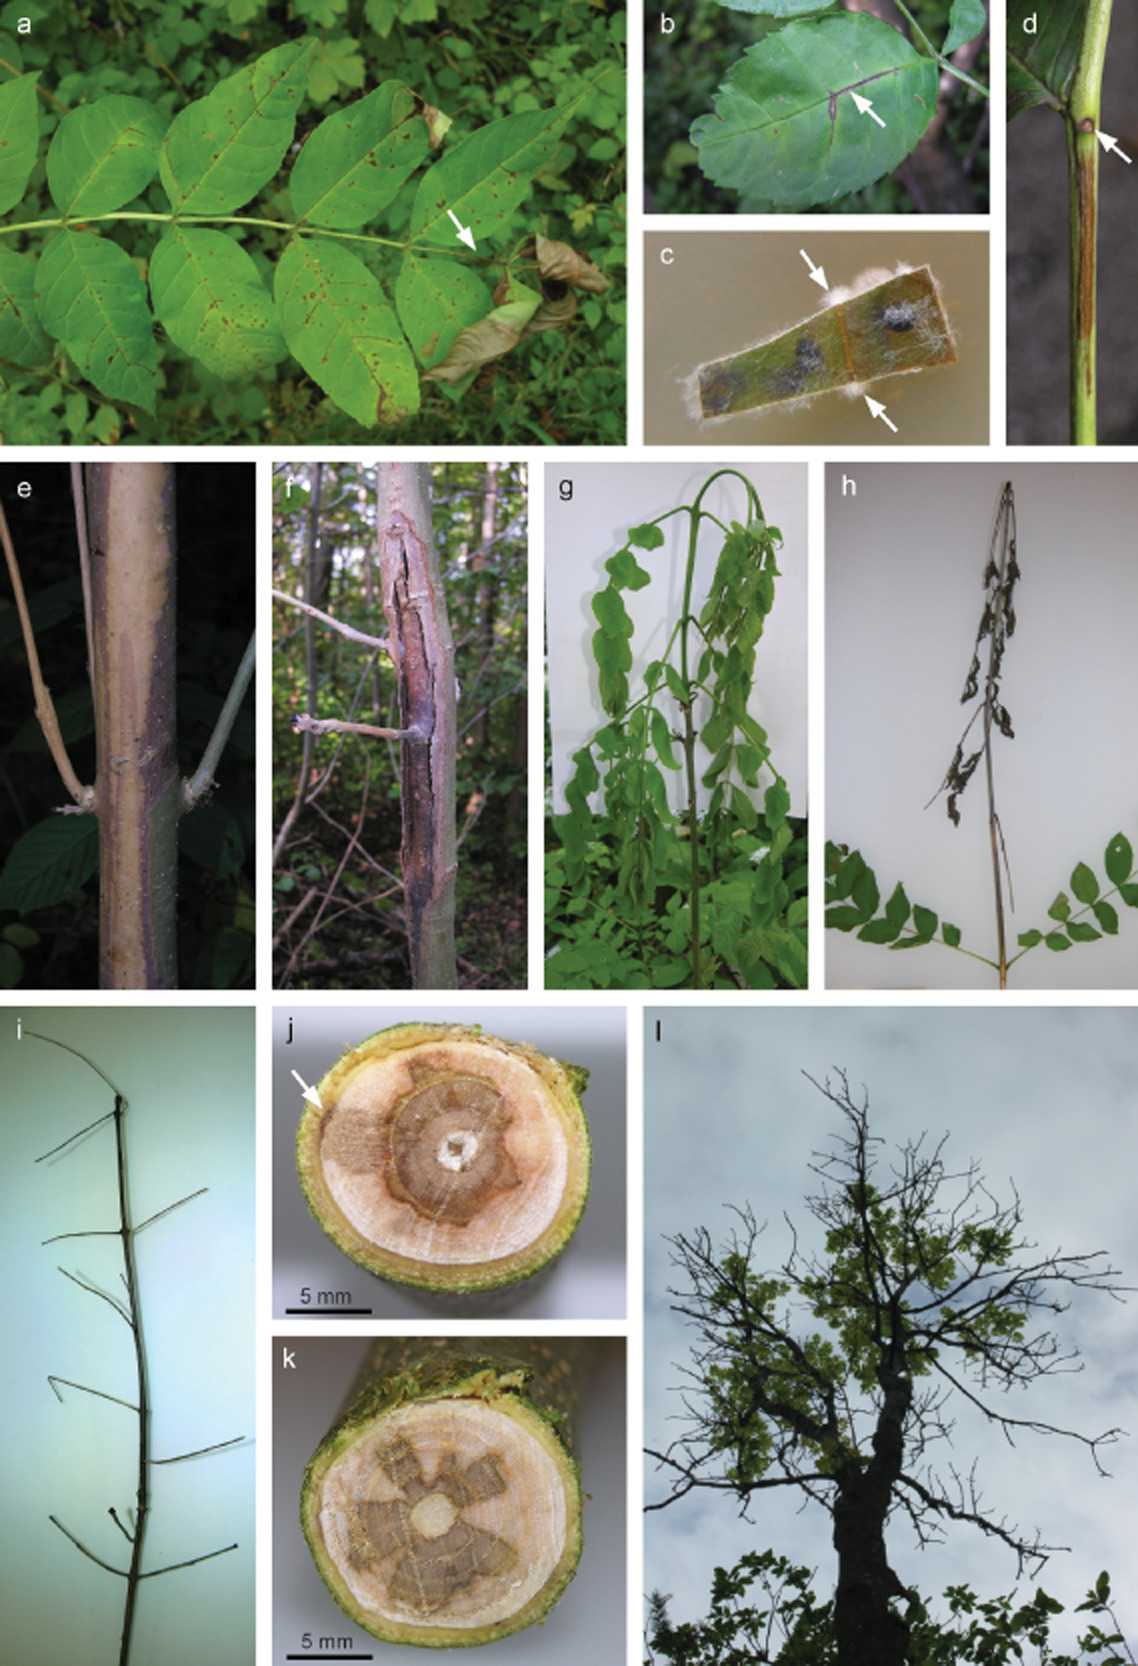
\includegraphics[scale=0.5]{chapter2/figures/gross2014.jpg}
    \caption{
    The symptoms of ash dieback, taken from the work of \cite{gross2014h}. 
    The pathogen \textit{H. fraxineus} infects the leaves of ash, leading to early onset wilting and desiccation. 
    The fungus then reproduces asexually, spreading through twigs, branches and eventually the xylem. 
    Symptoms include wilting, necrotic lesions, crown dieback and eventual mortality.}
    \label{fig:ash-deiback-symptoms}
\end{figure}

The pathogen HF is lethal to European ash of all ages. 
Nevertheless, research has established that small young ash trees are more at risk,
and susceptibility declines with maturity. Surveys of ash stands conducted by \cite{marccais2017estimation} 
in Belgium recorded that after six years of infection, small young saplings died with $35\%$ mortality, 
whilst slightly larger ash ($<25 \mathrm{cm}$ in diameter) displayed mortality of $11\%$. 
In contrast only $3.2\%$ of large mature ash ($>25\mathrm{cm}$ in diameter) died.

Various sources of ash mortality data have been collected in different European countries;
in Germany, a forest stand of planted ash trees showed a $73\%$
mortality rate after five years \cite{langer2015ash} (as cited in a review
\cite{enderle2017ash}), while observations of ADB progression in Austria
suggest a low mortality rate of $5\%$ measured over a two-year window \cite{kessler2012dieback}. 
A study conducted at different sites throughout Great Britain suggests a time scale ranging between 
$3-15$ years of infected tree growth before death \cite{wylder2018evidence}.

In addition to age, ash survival also depends on the landscape. 
Landscape features and ADB progression were studied by \cite{https://doi.org/10.1111/1365-2745.13383} 
over a sample plot of size  $\mathrm{3.5km \times 6.5 km}$ in France; observations over two years
suggest that the surrounding landscape has little impact initially in $2012$. However, after pathogen establishment, 
later surveys in $2016$-$2018$ showed that landscape features play an essential role.
Among the results put forward by \cite{https://doi.org/10.1111/1365-2745.13383}, 
a highly abundant ash region increased the prevalence of collar canker and rachis symptoms in neighbouring ash.
In addition, the authors found that the influence of ADB decayed exponentially up to $200-300\mathrm{m}$ away from the high density source,
thus suggesting a density-dependency in ADB spread.

Modelling work suggests a myriad of environmental factors can also predict the
vulnerability of ash and subsequent spread of disease \cite{dal2014risk}.
Spatial regression analysis conducted by \cite{chumanova2019predicting} in the Czech Republic indicates that altitude 
is an important predictor of pathogen growth, which also support the strong negative temperature dependence observed by \cite{hauptman2013temperature}.

\subsection{Life cycle and reproductive mode}
% WIKI: Hymenoscyphus fraxineus has two phases to its life-cycle: sexual and asexual.[9] The asexual stage (anamorph) grows in affected trees attacking the bark and encircling twigs and branches.[9] The sexual, reproductive stage, (teleomorph) grows during summer on ash petioles in the previous year's fallen leaves.[7] The ascospores are produced in asci and are transmitted by wind; this might explain the rapid spread of the fungus.[

The reproductive mode is intricate, and HF can infect hosts through the soil,
water, and air \cite{gross2012reproductive}; 
although, the primary natural driver of disease propagation is through wind-dispersal
during summertime sporulation. Sporulation typically occurs from June-September when 
fungal fruiting bodies on the previous litter-fall release ascospores \cite{grosdidier2018tracking, hietala2013invasive}.
Multiple ascospores sources can infect the same leaf \cite{gross2012reproductive}. 
Though the primary natural driver is wind, infection (and re-infection) of ash are also thought to be possible 
through the soil-borne mechanisms \cite{fones2016role}, albeit with low frequency.

\begin{figure}
    \centering
    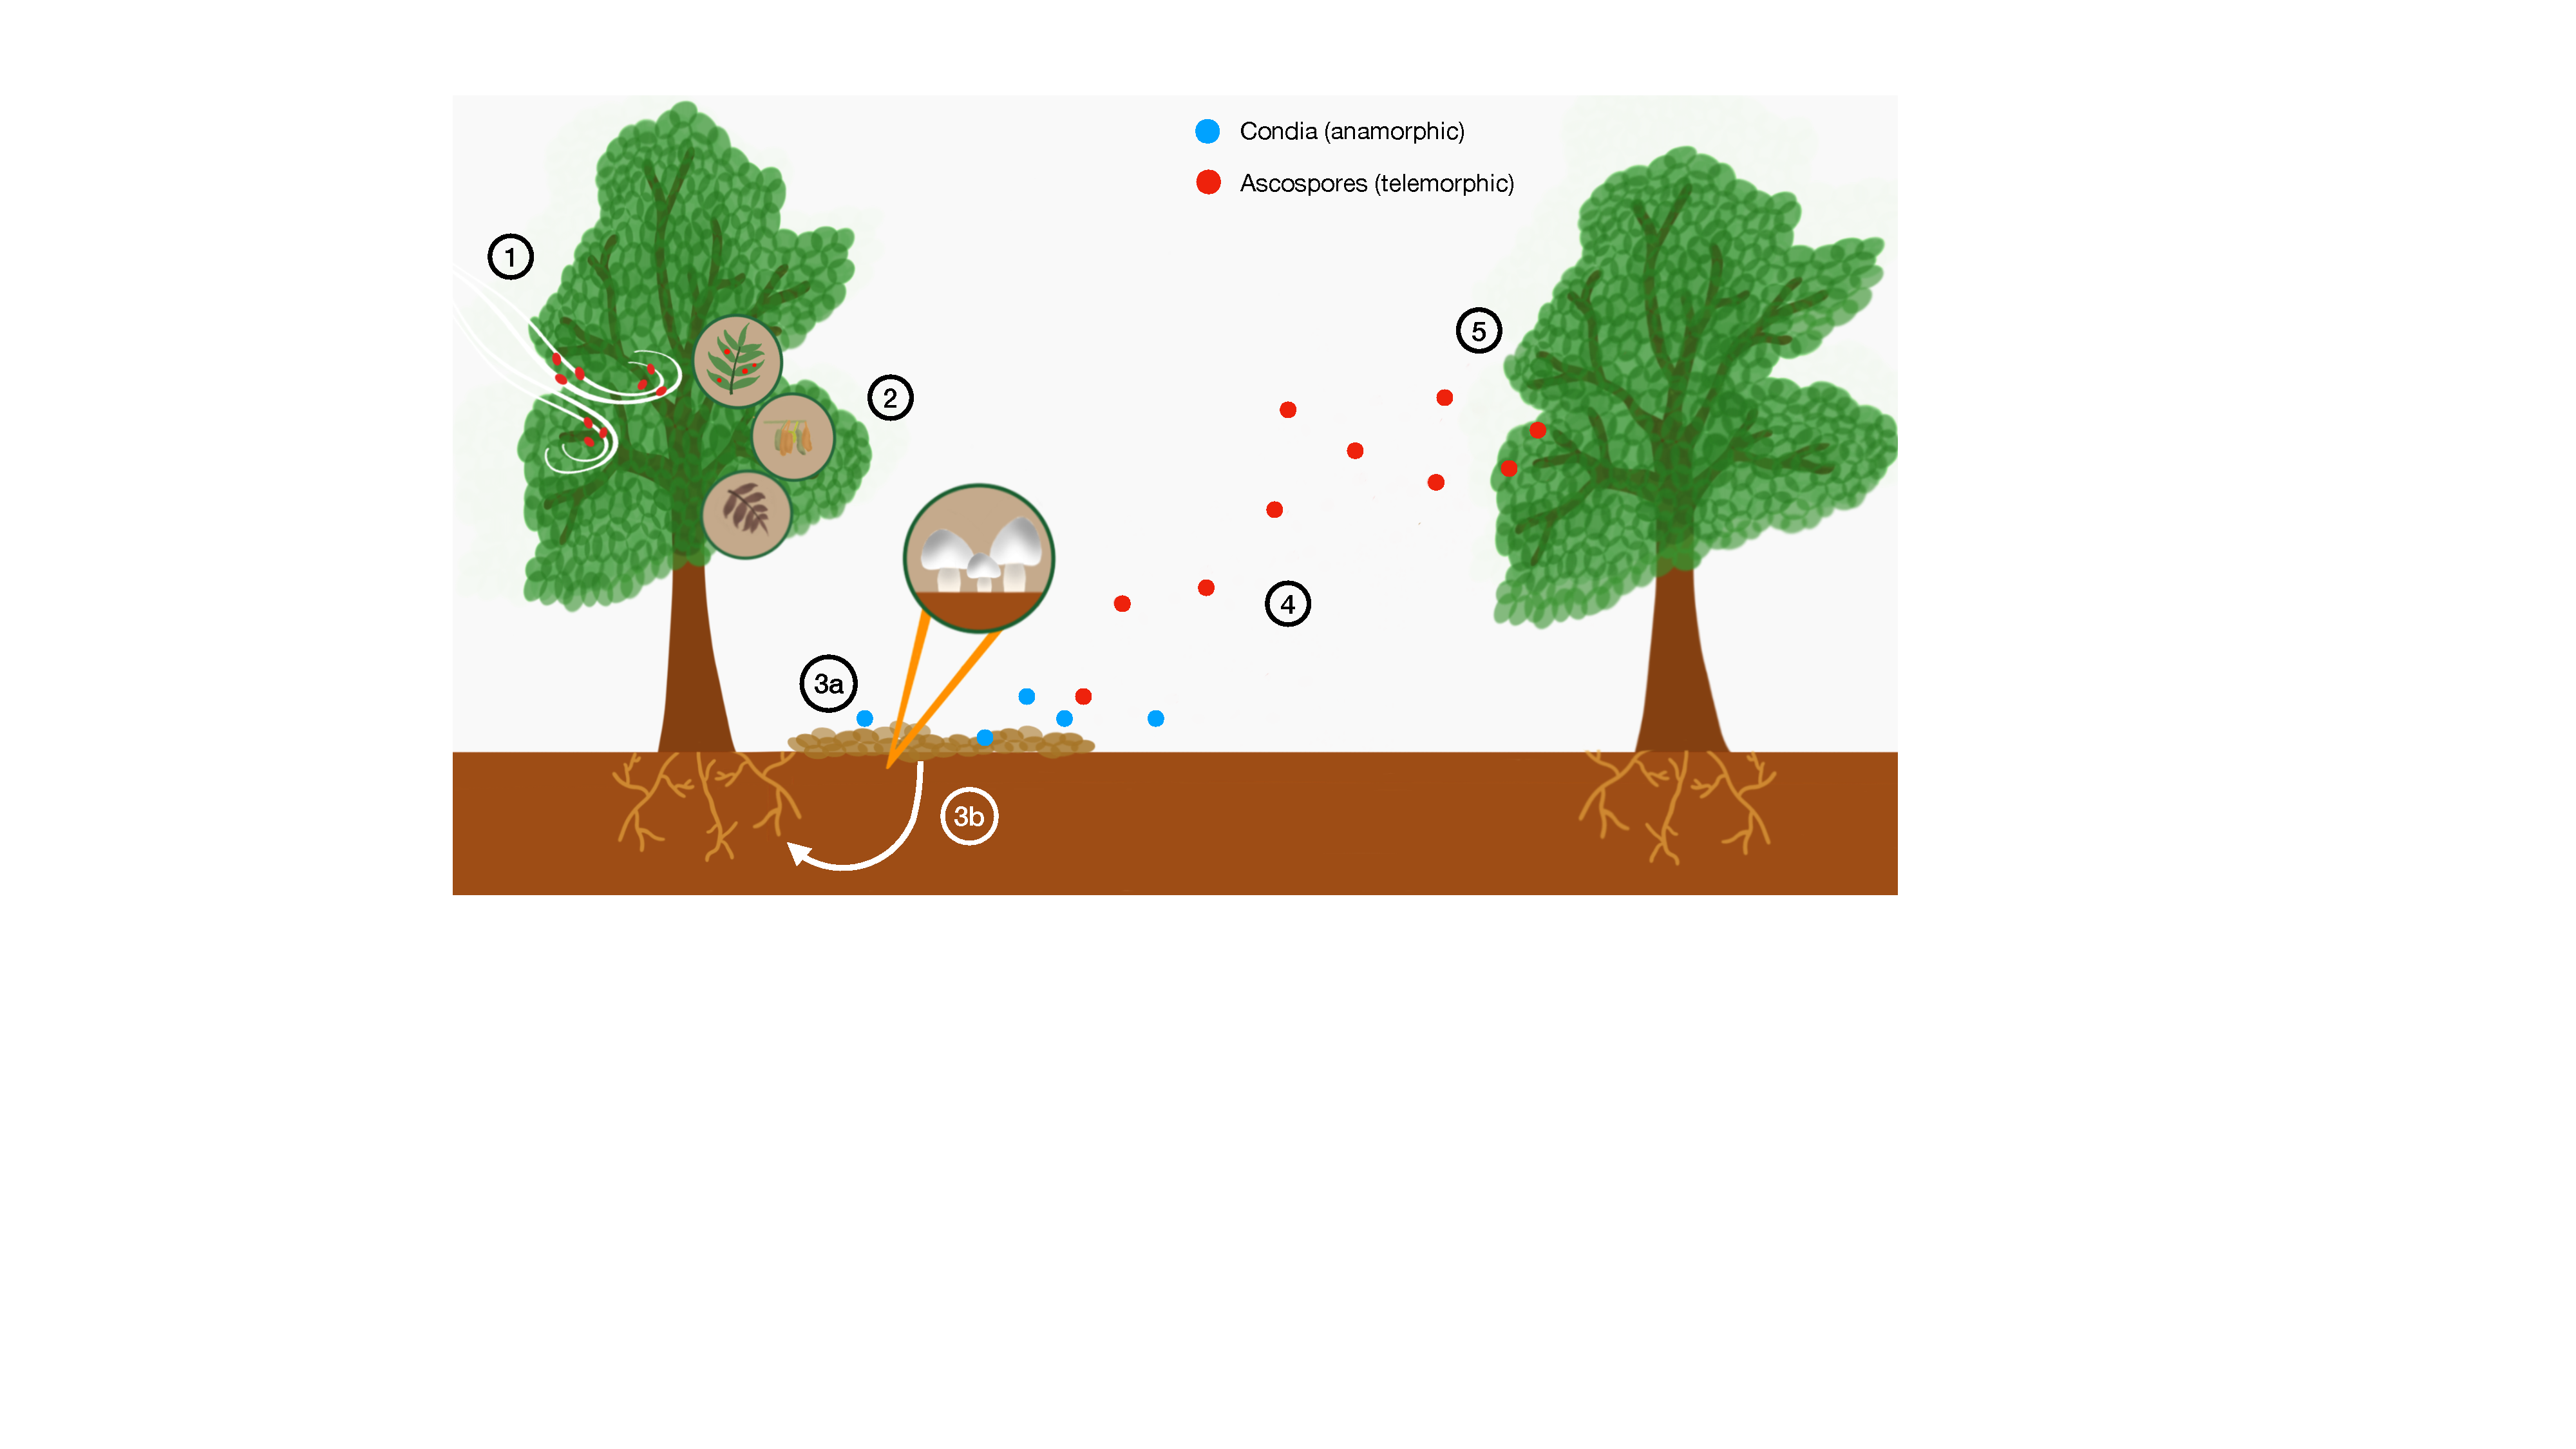
\includegraphics[scale=0.425]{chapter2/figures/ash-dieback-illustration.pdf}
    \caption{A life-cycle illustration of ADB: 
    1) HF ascospores disperse through wind during summertime sporulation, generally between June-September.
    Ascospore production constitutes HF's sexual (or `teleomorphic') reproduction mechanism.
    2) Ascospores penetrate the leaves of susceptible ash, causing the leaves to wilt.
       After spores infect leaves, the fungus proceeds to spread through twigs, branches and eventually the xylem.
       Infected leaves are shed in autumn, or from disease induced death.
    3a) Over winter, a mushroom-like fruiting body grows on infected leaf-fall (usually the petiole).
    3b) A proposed soil-borne infection mechanism has been proposed \cite{fones2016role}.
        Here, asexually reproducing HF mycelium are thought to infect the roots of ash trees.
    Through both steps 3a) and 3b), asexual condia disperse from the infected litterfall, shown in blue.
    Condia are proposed to act as spermatia, increasing the genetic diversity of HF.
    4) During the next summer period, immense numbers of ascospores are release from the fruiting body
    and disperse through wind.
    5) Ascospore dispersal induces ADB infections in distant susceptible ash. Fungal spores in particular 
    are known to travel large distances.
    }
    \label{fig:my_label}
\end{figure}

Ash dieback is highly seasonal \cite{bengtsson2014seasonal} and follows a complex, yearly polycyclic infection cycle.
Infected ash hosts will shed their leaves in the autumn, proceeded by fungal fruiting bodies growing on the dead leaf litter until summertime.
In summer, fruiting body spores are wind-dispersed and continue the cycle by producing new secondary infections\textemdash 
together, the life cycle and symptom expressions are illustrated in Figure \ref{fig:ash-deiback-symptoms}.
It is interesting to note the cyclic similarities between yearly ADB infection/re-infection and the seasonal
infections due to crop rotations, e.g. \cite{tankam2020modelling}. 
Notwithstanding that infected crop removal usually coincides with harvest time instead of infected ash survival that can span years.

The life cycle of the fungus HF can be understood to have two well-differentiated reproductive modes, 
sexual and asexual\textemdash a common trait of phyla Ascomycota, or ascomycetes fungi \cite{hawker2016physiology}.
Initially, asexual spores (conidia) were hypothesised to only increase genetic variance and act as spermatia \cite{gross2014h};
however \cite{fones2016role} called this into question, suggesting instead that asexual reproduction of the pathogen 
may play a role in driving the pathogen spread. Despite the potentially significant claim put forward by \cite{fones2016role},
it has gained seemingly little traction, and the role of asexual reproduction is still not fully understood.

\subsection{Dispersal}

In general, fungal spores have an efficient multi-scale wind-dispersal mechanism,
known to travel large distances \cite{golan2017long, wingen2013long, mundt2009aerial}
often described by power-law kernels, e.g. \cite{shaw2006assembling}.
From an epidemiological perspective, data on spore dispersal does not necessarily reflect the dynamics of new infections, 
as we cannot guarantee the availability of susceptible host material.
Even supposing available hosts, we cannot guarantee invasive spore colonisation.
However, studies on spore dispersal shed essential light on the spatial scale of ADB dispersal. 

Modern methods typically rely on `spore trapping' and real-time polymerase chain reaction (PCR) to study spores dispersal.
Data collected by \cite{chandelier2014detection} over three years using a (rotating arm) trapping system
and PRC amplification. The authors reported a $10\%$ spore trapping efficiency, and that most
dispersed ascospores remained within $50\mathrm{m}$ from the infectious source, with only a small number of spores exceeding 
distances beyond $50\mathrm{m}$. The work of \cite{chandelier2014detection} demonstrated the utility of novel PCR methods
to spore trap, but undesirably collected dispersal data over relatively small spatial scales.

Among the first landscape-scale fungal spore studies were conducted by \cite{long-range-dispersal}.
The authors focused on a comparable ascomycete fungus, \textit{Mycosphaerella fijiensis}, affecting banana plants.
Interestingly, \cite{long-range-dispersal} reported that asexual spore dispersal gradients extended 
a small distance $15\mathrm{m}$. As opposed to occasional, rare LDD in sexual (ascospore) dispersal up to $1000\mathrm{m}$.
Contrasting sexual and asexual spore dispersal was novel, and observing a small localised asexual dispersal gradient supports
the accepted idea that sexual dispersal in ADB is the dominant driver of disease spread.

Arguably the most comprehensive multi-scale study of ADB spore dispersal was performed by \cite{grosdidier2018tracking}.
In their paper, \cite{grosdidier2018tracking} tracked the local and landscape-level dispersal of ascospores
produced by \textit{H. fraxineus} in France.
The data collected relied on spore trapping and PRC; the reported trapping efficiency was $30–47\%$, marking an improvement over previous studies
e.g \cite{chandelier2014detection}. Most spores dispersal remained localised up to $50\mathrm{m}$ away from the inoculum source,
consistent with the results mentioned above put forward by \cite{chandelier2014detection}.
Nevertheless \cite{grosdidier2018tracking} set spore traps over much larger spatial scales ($\sim 100\mathrm{km}$),
subsequently detecting ADB spores $50-100\mathrm{km}$ ahead of the disease front.

Two dispersal kernels were used by \cite{grosdidier2018tracking}, a thin tailed Gaussian and an inverse 
power law of the forms:
\begin{equation}
    D(a, r) = \frac{1}{\pi a^2}\exp\big[-\frac{r^2}{a^2}\big]
    \label{eq:adb-ga}
\end{equation}
and
\begin{equation}
    D(a, r) = \frac{(b-1)(b-2)}{2\pi a^2}\big[ 1+ \frac{r}{a}\big]^{-b}
    \label{eq:geometric-invserse-power-law}
\end{equation}
where $a$ and $b$ are fitted parameters (for the Gaussian kernel, $a=\sqrt{2}\sigma$ with $\sigma$ being the standard deviation.).
In Equation \ref{eq:adb-ga}, the fitted value was $a=196\mathrm{m}$, while the fitted values in
Equation \ref{eq:geometric-invserse-power-law} were $a=203\mathrm{m}$ and $b=3.3$ respectively.

Equation \ref{eq:geometric-invserse-power-law} falls into the classical two-parameter geometric family of dispersal distributions.
The scale parameter is described by $a$ and the shape parameter by $b$. The mean dispersal distance described by Equation
\ref{eq:geometric-invserse-power-law} is $\frac{2a}{b-3}$, and parameters $a$ and $b$ are valid for $a>0$ and $b>2$.

The functional form of Equation \ref{eq:geometric-invserse-power-law} is predicated on pollen dispersal studies,
as reviewed by \cite{nathan2012dispersal}. The tail of Equation \ref{eq:geometric-invserse-power-law} is 
particularly well suited to describe LDD events, as noted by \cite{https://doi.org/10.1111/j.1365-294X.2004.02100.x}
when describing the dispersal of pollen particulates. Moreover, a study by \cite{https://doi.org/10.1111/j.1365-294X.2006.03155.x}
used Equation \ref{eq:geometric-invserse-power-law} to model pollen-dispersal (and thus plant gene-flow) over landscape-level spatial scales. 
Presumably, the ability of Equation \ref{eq:geometric-invserse-power-law} to describe LDD, and the size similarity between pollen and fungi spores, 
motivated \cite{grosdidier2018tracking} to include it their field study. 
% A recent article published by \cite{golan2017long} presents an interesting system to 

\subsection{Management and control}

Losing abundant ash populations could have dire consequences for several ecosystem functions, 
including nutrient recycling, food webs, and biodiversity.
As such, ADB presents a conservation challenge throughout Europe and Great Britain \cite{pautasso2013european}.
Moreover, under the rapid proliferation of ADB, various ash-dependent species risk extinction;
\cite{hultberg2020ash} identified $115$ at-risk (lichens, fungi, invertebrates, bryophytes/moss) species in Sweden that rely on ash.
Alarmingly, many of the ash-associated species identified by \cite{hultberg2020ash} also depend on elm species, which in turn face 
the fungal pathogen Dutch elm disease \cite{brasier1991ophiostoma}.

Given the ecological importance of ash in numerous temperate European forest types (e.g. floodplain, ravine, 
and lowland \cite{dobrowolska2011review}), management and pathogen control remain essential. The control of ash dieback
in a well-established focus of infestation, in both natural and artificial environments, is virtually impossible
\cite{havrdova2017environmental}, and it is already well recognised that ADB will eventually wipe out the vast 
majority of ash in Great Britain \cite{ash-dieback-costs}.

Controlling the spread of ash dieback reflects the spatial and temporal scale over which it spreads.
In particular, ADB fungal spores are thought to be able to jump between patches of ash,
even in the absence of susceptible hosts \cite{wingen2013long}.
However, LDD accounts for only a small minority of spore dispersal.
Furthermore, despite many notions of LDD, no unified LDD classification system exist, 
which led \cite{golan2017long} to propose a definition based on the distance traversed by the top $1\%$ of spores.

The long-term survival of ash depends on a small proportion of genetically resistant ash trees.
Despite many unpublished reports, genetic tolerance studies only began surfacing around a decade
after the widespread outbreak \cite{kjaer2012adaptive, stener2013clonal, mckinney2014ash}.
In particular, \cite{doi:10.1094/PHYTO-11-15-0284-R} showed the heritability of crown dieback and
collar-lesion symptom expression. In the three French provenances sampled,
\cite{doi:10.1094/PHYTO-11-15-0284-R} found no evidence for regional tolerance.
Presently, genetic tolerance is widely accepted \cite{havrdova2016differences, skovsgaard2017silvicultural},
and more recent work has focused on metabolomic tolerance classification,
profiling which metabolite markers correlate with resistance 
\cite{nemesio2020canditate, nemesio2020metabolomics, sidda2020diversity, chaudhary2020identification}.

A silvicultural system proposed by \cite{skovsgaard2017silvicultural} involves visually scoring severity based on crown dieback
and collar lesions. In this scheme, forest managers would inspect disease severity to record disease progression over time
and record genetically resistant trees to cultivate for future timber production. In addition, 
\cite{skovsgaard2017silvicultural} proposed that diseased forest stands should not be indiscriminately felled on account of high-value
tolerant individuals; this suggestion stands in contrast to the idea of a `cull radius', as alluded to by \cite{WEBIDEMICS}. 
In general, felling infected stands is ill-advised  \cite{chandelier2017ash}, except when infected hosts present a risk of uncontrolled 
and damaging tree-fall\textemdash as explained by \cite{ash-dieback-costs} when assessing the clean-up cost within Great Britain.

Following the establishment of genetic tolerance, numerous long-term preservation strategies 
rest on cultivating and replanting trees that exhibit low damage levels. Breeding 
programs in many European countries are currently underway, as reviewed by \cite{https://doi.org/10.1002/ppp3.10060}.
In the UK, the Living Tree Project (https://livingashproject.org.uk) aims to collate tolerant UK ash for future breeding.

% \cite{ash-tree2}
% - Approaches to conservation differ between forest and commercial ash stand \cite{skovsgaard2017silvicultural}. 
% - Among the control strategies, application of fungicide to infected biomass has been shown effective \cite{hauptman2015application}
% Among LDD human-mediated.
% - read me ->

% - statistical modelling work has shown the importance of environmental factors in the spread of disease \cite{dal2014risk, chumanova2019predicting}
% - the risk of spread.. was conduced by \cite{fellenor2019ash}....
% - \cite{dal2015epidemiology} un-published thesis